\documentclass[twoside]{book}

% Packages required by doxygen
\usepackage{fixltx2e}
\usepackage{calc}
\usepackage{doxygen}
\usepackage[export]{adjustbox} % also loads graphicx
\usepackage{graphicx}
\usepackage[utf8]{inputenc}
\usepackage{makeidx}
\usepackage{multicol}
\usepackage{multirow}
\PassOptionsToPackage{warn}{textcomp}
\usepackage{textcomp}
\usepackage[nointegrals]{wasysym}
\usepackage[table]{xcolor}

% Font selection
\usepackage[T1]{fontenc}
\usepackage[scaled=.90]{helvet}
\usepackage{courier}
\usepackage{amssymb}
\usepackage{sectsty}
\renewcommand{\familydefault}{\sfdefault}
\allsectionsfont{%
  \fontseries{bc}\selectfont%
  \color{darkgray}%
}
\renewcommand{\DoxyLabelFont}{%
  \fontseries{bc}\selectfont%
  \color{darkgray}%
}
\newcommand{\+}{\discretionary{\mbox{\scriptsize$\hookleftarrow$}}{}{}}

% Page & text layout
\usepackage{geometry}
\geometry{%
  a4paper,%
  top=2.5cm,%
  bottom=2.5cm,%
  left=2.5cm,%
  right=2.5cm%
}
\tolerance=750
\hfuzz=15pt
\hbadness=750
\setlength{\emergencystretch}{15pt}
\setlength{\parindent}{0cm}
\setlength{\parskip}{3ex plus 2ex minus 2ex}
\makeatletter
\renewcommand{\paragraph}{%
  \@startsection{paragraph}{4}{0ex}{-1.0ex}{1.0ex}{%
    \normalfont\normalsize\bfseries\SS@parafont%
  }%
}
\renewcommand{\subparagraph}{%
  \@startsection{subparagraph}{5}{0ex}{-1.0ex}{1.0ex}{%
    \normalfont\normalsize\bfseries\SS@subparafont%
  }%
}
\makeatother

% Headers & footers
\usepackage{fancyhdr}
\pagestyle{fancyplain}
\fancyhead[LE]{\fancyplain{}{\bfseries\thepage}}
\fancyhead[CE]{\fancyplain{}{}}
\fancyhead[RE]{\fancyplain{}{\bfseries\leftmark}}
\fancyhead[LO]{\fancyplain{}{\bfseries\rightmark}}
\fancyhead[CO]{\fancyplain{}{}}
\fancyhead[RO]{\fancyplain{}{\bfseries\thepage}}
\fancyfoot[LE]{\fancyplain{}{}}
\fancyfoot[CE]{\fancyplain{}{}}
\fancyfoot[RE]{\fancyplain{}{\bfseries\scriptsize Generated by Doxygen }}
\fancyfoot[LO]{\fancyplain{}{\bfseries\scriptsize Generated by Doxygen }}
\fancyfoot[CO]{\fancyplain{}{}}
\fancyfoot[RO]{\fancyplain{}{}}
\renewcommand{\footrulewidth}{0.4pt}
\renewcommand{\chaptermark}[1]{%
  \markboth{#1}{}%
}
\renewcommand{\sectionmark}[1]{%
  \markright{\thesection\ #1}%
}

% Indices & bibliography
\usepackage{natbib}
\usepackage[titles]{tocloft}
\setcounter{tocdepth}{3}
\setcounter{secnumdepth}{5}
\makeindex

% Hyperlinks (required, but should be loaded last)
\usepackage{ifpdf}
\ifpdf
  \usepackage[pdftex,pagebackref=true]{hyperref}
\else
  \usepackage[ps2pdf,pagebackref=true]{hyperref}
\fi
\hypersetup{%
  colorlinks=true,%
  linkcolor=blue,%
  citecolor=blue,%
  unicode%
}

% Custom commands
\newcommand{\clearemptydoublepage}{%
  \newpage{\pagestyle{empty}\cleardoublepage}%
}

\usepackage{caption}
\captionsetup{labelsep=space,justification=centering,font={bf},singlelinecheck=off,skip=4pt,position=top}

%===== C O N T E N T S =====

\begin{document}

% Titlepage & ToC
\hypersetup{pageanchor=false,
             bookmarksnumbered=true,
             pdfencoding=unicode
            }
\pagenumbering{alph}
\begin{titlepage}
\vspace*{7cm}
\begin{center}%
{\Large game-\/engine }\\
\vspace*{1cm}
{\large Generated by Doxygen 1.8.13}\\
\end{center}
\end{titlepage}
\clearemptydoublepage
\pagenumbering{roman}
\tableofcontents
\clearemptydoublepage
\pagenumbering{arabic}
\hypersetup{pageanchor=true}

%--- Begin generated contents ---
\chapter{Hierarchical Index}
\doxysection{Class Hierarchy}
This inheritance list is sorted roughly, but not completely, alphabetically\+:\begin{DoxyCompactList}
\item \contentsline{section}{engine\+::Application}{\pageref{classengine_1_1Application}}{}
\item \contentsline{section}{Application}{\pageref{classApplication}}{}
\item \contentsline{section}{engine\+::renderer\+::Buffer\+Element}{\pageref{structengine_1_1renderer_1_1BufferElement}}{}
\item \contentsline{section}{engine\+::renderer\+::Buffer\+Layout}{\pageref{classengine_1_1renderer_1_1BufferLayout}}{}
\item \contentsline{section}{engine\+::events\+::Event}{\pageref{classengine_1_1events_1_1Event}}{}
\begin{DoxyCompactList}
\item \contentsline{section}{engine\+::events\+::App\+Render\+Event}{\pageref{classengine_1_1events_1_1AppRenderEvent}}{}
\item \contentsline{section}{engine\+::events\+::App\+Tick\+Event}{\pageref{classengine_1_1events_1_1AppTickEvent}}{}
\item \contentsline{section}{engine\+::events\+::App\+Update\+Event}{\pageref{classengine_1_1events_1_1AppUpdateEvent}}{}
\item \contentsline{section}{engine\+::events\+::Key\+Event}{\pageref{classengine_1_1events_1_1KeyEvent}}{}
\begin{DoxyCompactList}
\item \contentsline{section}{engine\+::events\+::Key\+Pressed\+Event}{\pageref{classengine_1_1events_1_1KeyPressedEvent}}{}
\item \contentsline{section}{engine\+::events\+::Key\+Released\+Event}{\pageref{classengine_1_1events_1_1KeyReleasedEvent}}{}
\item \contentsline{section}{engine\+::events\+::Key\+Typed\+Event}{\pageref{classengine_1_1events_1_1KeyTypedEvent}}{}
\end{DoxyCompactList}
\item \contentsline{section}{engine\+::events\+::Mouse\+Button\+Event}{\pageref{classengine_1_1events_1_1MouseButtonEvent}}{}
\begin{DoxyCompactList}
\item \contentsline{section}{engine\+::events\+::Mouse\+Button\+Pressed\+Event}{\pageref{classengine_1_1events_1_1MouseButtonPressedEvent}}{}
\item \contentsline{section}{engine\+::events\+::Mouse\+Button\+Released\+Event}{\pageref{classengine_1_1events_1_1MouseButtonReleasedEvent}}{}
\end{DoxyCompactList}
\item \contentsline{section}{engine\+::events\+::Mouse\+Moved\+Event}{\pageref{classengine_1_1events_1_1MouseMovedEvent}}{}
\item \contentsline{section}{engine\+::events\+::Mouse\+Scrolled\+Event}{\pageref{classengine_1_1events_1_1MouseScrolledEvent}}{}
\item \contentsline{section}{engine\+::events\+::Window\+Close\+Event}{\pageref{classengine_1_1events_1_1WindowCloseEvent}}{}
\item \contentsline{section}{engine\+::events\+::Window\+Resize\+Event}{\pageref{classengine_1_1events_1_1WindowResizeEvent}}{}
\end{DoxyCompactList}
\item \contentsline{section}{engine\+::events\+::Event\+Dispatcher}{\pageref{classengine_1_1events_1_1EventDispatcher}}{}
\item \contentsline{section}{engine\+::renderer\+::Graphics\+Context}{\pageref{classengine_1_1renderer_1_1GraphicsContext}}{}
\begin{DoxyCompactList}
\item \contentsline{section}{engine\+::platform\+::opengl\+::Open\+G\+L\+Context}{\pageref{classengine_1_1platform_1_1opengl_1_1OpenGLContext}}{}
\end{DoxyCompactList}
\item \contentsline{section}{engine\+::renderer\+::Index\+Buffer}{\pageref{classengine_1_1renderer_1_1IndexBuffer}}{}
\begin{DoxyCompactList}
\item \contentsline{section}{engine\+::platform\+::opengl\+::Open\+G\+L\+Index\+Buffer}{\pageref{classengine_1_1platform_1_1opengl_1_1OpenGLIndexBuffer}}{}
\end{DoxyCompactList}
\item \contentsline{section}{engine\+::Input}{\pageref{classengine_1_1Input}}{}
\item \contentsline{section}{engine\+::Layer}{\pageref{classengine_1_1Layer}}{}
\begin{DoxyCompactList}
\item \contentsline{section}{engine\+::imgui\+::Im\+Gui\+Layer}{\pageref{classengine_1_1imgui_1_1ImGuiLayer}}{}
\end{DoxyCompactList}
\item \contentsline{section}{engine\+::Layer\+Stack}{\pageref{classengine_1_1LayerStack}}{}
\item \contentsline{section}{engine\+::logging\+::Log}{\pageref{classengine_1_1logging_1_1Log}}{}
\item \contentsline{section}{engine\+::renderer\+::Orthographic\+Camera}{\pageref{classengine_1_1renderer_1_1OrthographicCamera}}{}
\item \contentsline{section}{engine\+::renderer\+::Render\+Command}{\pageref{classengine_1_1renderer_1_1RenderCommand}}{}
\item \contentsline{section}{engine\+::renderer\+::Renderer}{\pageref{classengine_1_1renderer_1_1Renderer}}{}
\item \contentsline{section}{engine\+::renderer\+::Renderer\+A\+PI}{\pageref{classengine_1_1renderer_1_1RendererAPI}}{}
\begin{DoxyCompactList}
\item \contentsline{section}{engine\+::platform\+::opengl\+::Open\+G\+L\+Renderer\+A\+PI}{\pageref{classengine_1_1platform_1_1opengl_1_1OpenGLRendererAPI}}{}
\end{DoxyCompactList}
\item \contentsline{section}{engine\+::util\+::Reverse$<$ Container $>$}{\pageref{classengine_1_1util_1_1Reverse}}{}
\item \contentsline{section}{engine\+::renderer\+::Shader}{\pageref{classengine_1_1renderer_1_1Shader}}{}
\begin{DoxyCompactList}
\item \contentsline{section}{engine\+::platform\+::opengl\+::Open\+G\+L\+Shader}{\pageref{classengine_1_1platform_1_1opengl_1_1OpenGLShader}}{}
\end{DoxyCompactList}
\item \contentsline{section}{Shader}{\pageref{classShader}}{}
\item \contentsline{section}{engine\+::util\+::Time}{\pageref{classengine_1_1util_1_1Time}}{}
\item \contentsline{section}{engine\+::util\+::Time\+Step}{\pageref{classengine_1_1util_1_1TimeStep}}{}
\item \contentsline{section}{engine\+::renderer\+::Vertex\+Array}{\pageref{classengine_1_1renderer_1_1VertexArray}}{}
\begin{DoxyCompactList}
\item \contentsline{section}{engine\+::platform\+::opengl\+::Open\+G\+L\+Vertex\+Array}{\pageref{classengine_1_1platform_1_1opengl_1_1OpenGLVertexArray}}{}
\end{DoxyCompactList}
\item \contentsline{section}{Vertex\+Array}{\pageref{classVertexArray}}{}
\item \contentsline{section}{engine\+::renderer\+::Vertex\+Buffer}{\pageref{classengine_1_1renderer_1_1VertexBuffer}}{}
\begin{DoxyCompactList}
\item \contentsline{section}{engine\+::platform\+::opengl\+::Open\+G\+L\+Vertex\+Buffer}{\pageref{classengine_1_1platform_1_1opengl_1_1OpenGLVertexBuffer}}{}
\end{DoxyCompactList}
\item \contentsline{section}{engine\+::Window}{\pageref{classengine_1_1Window}}{}
\item \contentsline{section}{engine\+::Window\+Properties}{\pageref{structengine_1_1WindowProperties}}{}
\end{DoxyCompactList}

\chapter{Class Index}
\doxysection{Class List}
Here are the classes, structs, unions and interfaces with brief descriptions\+:\begin{DoxyCompactList}
\item\contentsline{section}{\mbox{\hyperlink{classlambda_1_1core_1_1Application}{lambda\+::core\+::\+Application}} \\*The mind, body, and soul of Lambda. The \mbox{\hyperlink{classlambda_1_1core_1_1Application}{Application}} class is the }{\pageref{classlambda_1_1core_1_1Application}}{}
\item\contentsline{section}{\mbox{\hyperlink{classlambda_1_1core_1_1events_1_1AppRenderEvent}{lambda\+::core\+::events\+::\+App\+Render\+Event}} \\*An event generated when the app has rendered }{\pageref{classlambda_1_1core_1_1events_1_1AppRenderEvent}}{}
\item\contentsline{section}{\mbox{\hyperlink{classlambda_1_1core_1_1events_1_1AppTickEvent}{lambda\+::core\+::events\+::\+App\+Tick\+Event}} \\*An \mbox{\hyperlink{classlambda_1_1core_1_1events_1_1Event}{Event}} generated when the app has ticked }{\pageref{classlambda_1_1core_1_1events_1_1AppTickEvent}}{}
\item\contentsline{section}{\mbox{\hyperlink{classlambda_1_1core_1_1events_1_1AppUpdateEvent}{lambda\+::core\+::events\+::\+App\+Update\+Event}} \\*An event generated when the app has updated }{\pageref{classlambda_1_1core_1_1events_1_1AppUpdateEvent}}{}
\item\contentsline{section}{\mbox{\hyperlink{classlambda_1_1core_1_1io_1_1AsyncTask}{lambda\+::core\+::io\+::\+Async\+Task}} \\*A wrapper for callbacks that are supposed to be executed asynchronously }{\pageref{classlambda_1_1core_1_1io_1_1AsyncTask}}{}
\item\contentsline{section}{\mbox{\hyperlink{structlambda_1_1core_1_1renderer_1_1BufferElement}{lambda\+::core\+::renderer\+::\+Buffer\+Element}} \\*A generic buffer element used for describing the layout of a buffer }{\pageref{structlambda_1_1core_1_1renderer_1_1BufferElement}}{}
\item\contentsline{section}{\mbox{\hyperlink{classlambda_1_1core_1_1renderer_1_1BufferLayout}{lambda\+::core\+::renderer\+::\+Buffer\+Layout}} \\*The layout of a vertex buffer. Should always be instantiated with buffer elements for it to work properly }{\pageref{classlambda_1_1core_1_1renderer_1_1BufferLayout}}{}
\item\contentsline{section}{\mbox{\hyperlink{classlambda_1_1core_1_1events_1_1Event}{lambda\+::core\+::events\+::\+Event}} \\*The base \mbox{\hyperlink{classlambda_1_1core_1_1events_1_1Event}{Event}} class for events that are propagated throughout lambda }{\pageref{classlambda_1_1core_1_1events_1_1Event}}{}
\item\contentsline{section}{\mbox{\hyperlink{classlambda_1_1core_1_1events_1_1EventDispatcher}{lambda\+::core\+::events\+::\+Event\+Dispatcher}} \\*The primary way of allowing the application and layers in lambda the capability of handling events propagated throughout the application }{\pageref{classlambda_1_1core_1_1events_1_1EventDispatcher}}{}
\item\contentsline{section}{\mbox{\hyperlink{classlambda_1_1core_1_1io_1_1EventLoop}{lambda\+::core\+::io\+::\+Event\+Loop}} \\*Asynchronous Event Loop that allows the execution of code to happen in another thread. This is not recommended for production as of yet }{\pageref{classlambda_1_1core_1_1io_1_1EventLoop}}{}
\item\contentsline{section}{\mbox{\hyperlink{classlambda_1_1core_1_1util_1_1File}{lambda\+::core\+::util\+::\+File}} \\*T\+O\+D\+O(\+C3\+N\+Z)\+: Implement this for linux and (maybe) Windows system next }{\pageref{classlambda_1_1core_1_1util_1_1File}}{}
\item\contentsline{section}{\mbox{\hyperlink{classlambda_1_1core_1_1renderer_1_1GraphicsContext}{lambda\+::core\+::renderer\+::\+Graphics\+Context}} \\*The Graphics context abstraction }{\pageref{classlambda_1_1core_1_1renderer_1_1GraphicsContext}}{}
\item\contentsline{section}{\mbox{\hyperlink{classlambda_1_1core_1_1imgui_1_1ImGuiLayer}{lambda\+::core\+::imgui\+::\+Im\+Gui\+Layer}} \\*The base Im\+Gui layer used for rendering all other Im\+Gui components }{\pageref{classlambda_1_1core_1_1imgui_1_1ImGuiLayer}}{}
\item\contentsline{section}{\mbox{\hyperlink{classlambda_1_1core_1_1renderer_1_1IndexBuffer}{lambda\+::core\+::renderer\+::\+Index\+Buffer}} \\*A general abstraction of an Index Buffer }{\pageref{classlambda_1_1core_1_1renderer_1_1IndexBuffer}}{}
\item\contentsline{section}{\mbox{\hyperlink{classlambda_1_1core_1_1input_1_1Input}{lambda\+::core\+::input\+::\+Input}} \\*The generic input system for getting input data from applications built on lambda }{\pageref{classlambda_1_1core_1_1input_1_1Input}}{}
\item\contentsline{section}{\mbox{\hyperlink{classlambda_1_1core_1_1events_1_1KeyEvent}{lambda\+::core\+::events\+::\+Key\+Event}} \\*The Base Key \mbox{\hyperlink{classlambda_1_1core_1_1events_1_1Event}{Event}} used for other Key Events }{\pageref{classlambda_1_1core_1_1events_1_1KeyEvent}}{}
\item\contentsline{section}{\mbox{\hyperlink{classlambda_1_1core_1_1events_1_1KeyPressedEvent}{lambda\+::core\+::events\+::\+Key\+Pressed\+Event}} \\*An \mbox{\hyperlink{classlambda_1_1core_1_1events_1_1Event}{Event}} generated whenever a key is pressed within an application that is running lambda }{\pageref{classlambda_1_1core_1_1events_1_1KeyPressedEvent}}{}
\item\contentsline{section}{\mbox{\hyperlink{classlambda_1_1core_1_1events_1_1KeyReleasedEvent}{lambda\+::core\+::events\+::\+Key\+Released\+Event}} \\*An \mbox{\hyperlink{classlambda_1_1core_1_1events_1_1Event}{Event}} generated whenever a key is released within an application that is running lambda }{\pageref{classlambda_1_1core_1_1events_1_1KeyReleasedEvent}}{}
\item\contentsline{section}{\mbox{\hyperlink{classlambda_1_1core_1_1events_1_1KeyTypedEvent}{lambda\+::core\+::events\+::\+Key\+Typed\+Event}} \\*An \mbox{\hyperlink{classlambda_1_1core_1_1events_1_1Event}{Event}} generated whenever a key is typed within an application that is running lambda. (Keys typed do not track any repeat counts.) }{\pageref{classlambda_1_1core_1_1events_1_1KeyTypedEvent}}{}
\item\contentsline{section}{\mbox{\hyperlink{classlambda_1_1core_1_1layers_1_1Layer}{lambda\+::core\+::layers\+::\+Layer}} \\*The lambda \mbox{\hyperlink{classlambda_1_1core_1_1layers_1_1Layer}{Layer}} abstraction. Primarily used for direct access into lambdas tick and event system }{\pageref{classlambda_1_1core_1_1layers_1_1Layer}}{}
\item\contentsline{section}{\mbox{\hyperlink{classlambda_1_1core_1_1layers_1_1LayerStack}{lambda\+::core\+::layers\+::\+Layer\+Stack}} \\*A Stack based structure for lambda to manage layers in }{\pageref{classlambda_1_1core_1_1layers_1_1LayerStack}}{}
\item\contentsline{section}{\mbox{\hyperlink{classlambda_1_1core_1_1util_1_1Log}{lambda\+::core\+::util\+::\+Log}} \\*The container class for managing static instances of the engine and client loggers }{\pageref{classlambda_1_1core_1_1util_1_1Log}}{}
\item\contentsline{section}{\mbox{\hyperlink{classlambda_1_1core_1_1events_1_1MouseButtonEvent}{lambda\+::core\+::events\+::\+Mouse\+Button\+Event}} \\*The base event class for all events mouse button related }{\pageref{classlambda_1_1core_1_1events_1_1MouseButtonEvent}}{}
\item\contentsline{section}{\mbox{\hyperlink{classlambda_1_1core_1_1events_1_1MouseButtonPressedEvent}{lambda\+::core\+::events\+::\+Mouse\+Button\+Pressed\+Event}} \\*An event generated whenever a Mouse button is pressed within an application that is running lambda }{\pageref{classlambda_1_1core_1_1events_1_1MouseButtonPressedEvent}}{}
\item\contentsline{section}{\mbox{\hyperlink{classlambda_1_1core_1_1events_1_1MouseButtonReleasedEvent}{lambda\+::core\+::events\+::\+Mouse\+Button\+Released\+Event}} \\*An event generated whenever a Mouse button is released within an application that is running lambda }{\pageref{classlambda_1_1core_1_1events_1_1MouseButtonReleasedEvent}}{}
\item\contentsline{section}{\mbox{\hyperlink{classlambda_1_1core_1_1events_1_1MouseMovedEvent}{lambda\+::core\+::events\+::\+Mouse\+Moved\+Event}} \\*An event generated whenever a mouse is moved within an application that is running lambda }{\pageref{classlambda_1_1core_1_1events_1_1MouseMovedEvent}}{}
\item\contentsline{section}{\mbox{\hyperlink{classlambda_1_1core_1_1events_1_1MouseScrolledEvent}{lambda\+::core\+::events\+::\+Mouse\+Scrolled\+Event}} \\*An event generated whenever a mouse is scrolled within an application that is running lambda }{\pageref{classlambda_1_1core_1_1events_1_1MouseScrolledEvent}}{}
\item\contentsline{section}{\mbox{\hyperlink{classlambda_1_1platform_1_1opengl_1_1OpenGLContext}{lambda\+::platform\+::opengl\+::\+Open\+G\+L\+Context}} }{\pageref{classlambda_1_1platform_1_1opengl_1_1OpenGLContext}}{}
\item\contentsline{section}{\mbox{\hyperlink{classlambda_1_1platform_1_1opengl_1_1OpenGLIndexBuffer}{lambda\+::platform\+::opengl\+::\+Open\+G\+L\+Index\+Buffer}} }{\pageref{classlambda_1_1platform_1_1opengl_1_1OpenGLIndexBuffer}}{}
\item\contentsline{section}{\mbox{\hyperlink{classlambda_1_1platform_1_1opengl_1_1OpenGLRendererAPI}{lambda\+::platform\+::opengl\+::\+Open\+G\+L\+Renderer\+A\+PI}} \\*The Rendering implementation for Open\+GL }{\pageref{classlambda_1_1platform_1_1opengl_1_1OpenGLRendererAPI}}{}
\item\contentsline{section}{\mbox{\hyperlink{classlambda_1_1platform_1_1opengl_1_1OpenGLShader}{lambda\+::platform\+::opengl\+::\+Open\+G\+L\+Shader}} }{\pageref{classlambda_1_1platform_1_1opengl_1_1OpenGLShader}}{}
\item\contentsline{section}{\mbox{\hyperlink{classlambda_1_1platform_1_1opengl_1_1OpenGLTexture2D}{lambda\+::platform\+::opengl\+::\+Open\+G\+L\+Texture2D}} \\*The opengl 2D texture implementation }{\pageref{classlambda_1_1platform_1_1opengl_1_1OpenGLTexture2D}}{}
\item\contentsline{section}{\mbox{\hyperlink{classlambda_1_1platform_1_1opengl_1_1OpenGLVertexArray}{lambda\+::platform\+::opengl\+::\+Open\+G\+L\+Vertex\+Array}} \\*The abstraction for representing Vertex arrays and their sub components }{\pageref{classlambda_1_1platform_1_1opengl_1_1OpenGLVertexArray}}{}
\item\contentsline{section}{\mbox{\hyperlink{classlambda_1_1platform_1_1opengl_1_1OpenGLVertexBuffer}{lambda\+::platform\+::opengl\+::\+Open\+G\+L\+Vertex\+Buffer}} }{\pageref{classlambda_1_1platform_1_1opengl_1_1OpenGLVertexBuffer}}{}
\item\contentsline{section}{\mbox{\hyperlink{classlambda_1_1core_1_1renderer_1_1OrthographicCamera}{lambda\+::core\+::renderer\+::\+Orthographic\+Camera}} \\*An orthographic camera implementation for the 2D engine }{\pageref{classlambda_1_1core_1_1renderer_1_1OrthographicCamera}}{}
\item\contentsline{section}{\mbox{\hyperlink{classlambda_1_1core_1_1OrthographicCameraController}{lambda\+::core\+::\+Orthographic\+Camera\+Controller}} }{\pageref{classlambda_1_1core_1_1OrthographicCameraController}}{}
\item\contentsline{section}{\mbox{\hyperlink{classlambda_1_1core_1_1renderer_1_1RenderCommand}{lambda\+::core\+::renderer\+::\+Render\+Command}} \\*An interface for issuing commands to the current rendering A\+PI that is being used with lambda }{\pageref{classlambda_1_1core_1_1renderer_1_1RenderCommand}}{}
\item\contentsline{section}{\mbox{\hyperlink{classlambda_1_1core_1_1renderer_1_1Renderer}{lambda\+::core\+::renderer\+::\+Renderer}} \\*The primary interface used for managing }{\pageref{classlambda_1_1core_1_1renderer_1_1Renderer}}{}
\item\contentsline{section}{\mbox{\hyperlink{classlambda_1_1core_1_1renderer_1_1RendererAPI}{lambda\+::core\+::renderer\+::\+Renderer\+A\+PI}} \\*The abstract representation of rendering features and functions supported by Lambda }{\pageref{classlambda_1_1core_1_1renderer_1_1RendererAPI}}{}
\item\contentsline{section}{\mbox{\hyperlink{classlambda_1_1core_1_1util_1_1Reverse}{lambda\+::core\+::util\+::\+Reverse$<$ Container $>$}} \\*A clean container for iterating through any container that implements rbegin and rend }{\pageref{classlambda_1_1core_1_1util_1_1Reverse}}{}
\item\contentsline{section}{\mbox{\hyperlink{classlambda_1_1core_1_1renderer_1_1Shader}{lambda\+::core\+::renderer\+::\+Shader}} \\*A generic \mbox{\hyperlink{classlambda_1_1core_1_1renderer_1_1Shader}{Shader}} A\+PI }{\pageref{classlambda_1_1core_1_1renderer_1_1Shader}}{}
\item\contentsline{section}{\mbox{\hyperlink{classShader}{Shader}} \\*The \mbox{\hyperlink{classShader}{Shader}} A\+PI }{\pageref{classShader}}{}
\item\contentsline{section}{\mbox{\hyperlink{classlambda_1_1core_1_1renderer_1_1ShaderLibrary}{lambda\+::core\+::renderer\+::\+Shader\+Library}} \\*A library for managing many different shaders }{\pageref{classlambda_1_1core_1_1renderer_1_1ShaderLibrary}}{}
\item\contentsline{section}{\mbox{\hyperlink{classlambda_1_1core_1_1renderer_1_1Texture}{lambda\+::core\+::renderer\+::\+Texture}} \\*The abstract texture A\+PI }{\pageref{classlambda_1_1core_1_1renderer_1_1Texture}}{}
\item\contentsline{section}{\mbox{\hyperlink{classlambda_1_1core_1_1renderer_1_1Texture2D}{lambda\+::core\+::renderer\+::\+Texture2D}} \\*The 2D \mbox{\hyperlink{classlambda_1_1core_1_1renderer_1_1Texture}{Texture}} A\+PI }{\pageref{classlambda_1_1core_1_1renderer_1_1Texture2D}}{}
\item\contentsline{section}{\mbox{\hyperlink{classlambda_1_1core_1_1util_1_1Time}{lambda\+::core\+::util\+::\+Time}} }{\pageref{classlambda_1_1core_1_1util_1_1Time}}{}
\item\contentsline{section}{\mbox{\hyperlink{classlambda_1_1util_1_1Time}{Time}} \\*A wrapper for working with \mbox{\hyperlink{classlambda_1_1util_1_1Time}{Time}} within the game engine. Uses std\+::steady\+\_\+clock for a platform independent Monotonic clock }{\pageref{classlambda_1_1util_1_1Time}}{}
\item\contentsline{section}{\mbox{\hyperlink{classlambda_1_1core_1_1util_1_1TimeStep}{lambda\+::core\+::util\+::\+Time\+Step}} }{\pageref{classlambda_1_1core_1_1util_1_1TimeStep}}{}
\item\contentsline{section}{\mbox{\hyperlink{classlambda_1_1util_1_1TimeStep}{Time\+Step}} \\*The timestep between two time intervals. Primarily used for layers to consistently update the engine }{\pageref{classlambda_1_1util_1_1TimeStep}}{}
\item\contentsline{section}{\mbox{\hyperlink{classlambda_1_1core_1_1renderer_1_1VertexArray}{lambda\+::core\+::renderer\+::\+Vertex\+Array}} \\*The abstract \mbox{\hyperlink{classlambda_1_1core_1_1renderer_1_1VertexArray}{Vertex\+Array}} A\+PI }{\pageref{classlambda_1_1core_1_1renderer_1_1VertexArray}}{}
\item\contentsline{section}{\mbox{\hyperlink{classlambda_1_1core_1_1renderer_1_1VertexBuffer}{lambda\+::core\+::renderer\+::\+Vertex\+Buffer}} \\*A general abstraction of Vertex Buffer }{\pageref{classlambda_1_1core_1_1renderer_1_1VertexBuffer}}{}
\item\contentsline{section}{\mbox{\hyperlink{classlambda_1_1core_1_1Window}{lambda\+::core\+::\+Window}} }{\pageref{classlambda_1_1core_1_1Window}}{}
\item\contentsline{section}{\mbox{\hyperlink{classlambda_1_1Window}{Window}} \\*The generic window implementation that allows platform specific window A\+P\+Is to expose generic window functionality without users having to know the window system }{\pageref{classlambda_1_1Window}}{}
\item\contentsline{section}{\mbox{\hyperlink{classlambda_1_1core_1_1events_1_1WindowCloseEvent}{lambda\+::core\+::events\+::\+Window\+Close\+Event}} \\*An \mbox{\hyperlink{classlambda_1_1core_1_1events_1_1Event}{Event}} generated when the \mbox{\hyperlink{classlambda_1_1core_1_1Window}{Window}} has closed }{\pageref{classlambda_1_1core_1_1events_1_1WindowCloseEvent}}{}
\item\contentsline{section}{\mbox{\hyperlink{structlambda_1_1core_1_1WindowProperties}{lambda\+::core\+::\+Window\+Properties}} }{\pageref{structlambda_1_1core_1_1WindowProperties}}{}
\item\contentsline{section}{\mbox{\hyperlink{structlambda_1_1WindowProperties}{Window\+Properties}} \\*Generic \mbox{\hyperlink{classlambda_1_1Window}{Window}} properties used to create platform specific windows }{\pageref{structlambda_1_1WindowProperties}}{}
\item\contentsline{section}{\mbox{\hyperlink{classlambda_1_1core_1_1events_1_1WindowResizeEvent}{lambda\+::core\+::events\+::\+Window\+Resize\+Event}} \\*An \mbox{\hyperlink{classlambda_1_1core_1_1events_1_1Event}{Event}} generated when the \mbox{\hyperlink{classlambda_1_1core_1_1Window}{Window}} has resized }{\pageref{classlambda_1_1core_1_1events_1_1WindowResizeEvent}}{}
\end{DoxyCompactList}

\chapter{Class Documentation}
\hypertarget{classengine_1_1Application}{}\section{engine\+:\+:Application Class Reference}
\label{classengine_1_1Application}\index{engine\+::\+Application@{engine\+::\+Application}}


The primary driver of all applications extending this engine.  




{\ttfamily \#include $<$Application.\+h$>$}

\subsection*{Public Member Functions}
\begin{DoxyCompactItemize}
\item 
\hyperlink{classengine_1_1Application_a9740cd2e55318cbc5684a6c4c2f3304f}{Application} ()
\item 
void \hyperlink{classengine_1_1Application_a4dcdf08d920f7f63013a25cb1e80438b}{Run} ()
\begin{DoxyCompactList}\small\item\em Controls the applications lifecycle and all lower level functionality like input, events, rendering, networking, etc. \end{DoxyCompactList}\item 
void \hyperlink{classengine_1_1Application_a093e14152fc1eda1b5eba682a2b4afd9}{On\+Event} (\hyperlink{classengine_1_1events_1_1Event}{events\+::\+Event} $\ast$event)
\begin{DoxyCompactList}\small\item\em Passes events to all the layers. \end{DoxyCompactList}\item 
void \hyperlink{classengine_1_1Application_adb129a86a6cdbd80b25094d08605d213}{Push\+Layer} (\hyperlink{classengine_1_1Layer}{Layer} $\ast$layer)
\begin{DoxyCompactList}\small\item\em Attaches a layer to the application instance. \end{DoxyCompactList}\item 
\mbox{\Hypertarget{classengine_1_1Application_a8dab10f6982032021b2091e2a96fdfc2}\label{classengine_1_1Application_a8dab10f6982032021b2091e2a96fdfc2}} 
void \hyperlink{classengine_1_1Application_a8dab10f6982032021b2091e2a96fdfc2}{Push\+Overlay} (\hyperlink{classengine_1_1Layer}{Layer} $\ast$layer)
\begin{DoxyCompactList}\small\item\em Attaches an overlay to the application instance. This allows the application instance to propage events, renderine, and any desired pieces of data into the layer. \end{DoxyCompactList}\item 
const \hyperlink{classengine_1_1Window}{Window} \& \hyperlink{classengine_1_1Application_a0c66a3ff294bcc497bb2e8eb7330124c}{Get\+Window} () const
\end{DoxyCompactItemize}
\subsection*{Static Public Member Functions}
\begin{DoxyCompactItemize}
\item 
static \hyperlink{classengine_1_1Application}{Application} \& \hyperlink{classengine_1_1Application_a639cdab87d3c5a14d0a9e9203d6c7c97}{Get\+Application} ()
\end{DoxyCompactItemize}


\subsection{Detailed Description}
The primary driver of all applications extending this engine. 

The engine implements the application runner as an individual platform independent application instance that manages the lifecycle of the core and lower level components of the engine. 

\subsection{Constructor \& Destructor Documentation}
\mbox{\Hypertarget{classengine_1_1Application_a9740cd2e55318cbc5684a6c4c2f3304f}\label{classengine_1_1Application_a9740cd2e55318cbc5684a6c4c2f3304f}} 
\index{engine\+::\+Application@{engine\+::\+Application}!Application@{Application}}
\index{Application@{Application}!engine\+::\+Application@{engine\+::\+Application}}
\subsubsection{\texorpdfstring{Application()}{Application()}}
{\footnotesize\ttfamily engine\+::\+Application\+::\+Application (\begin{DoxyParamCaption}{ }\end{DoxyParamCaption})}

T\+O\+D\+O(\+C3\+N\+Z)\+: This should not carry as much of a load as it currently does and should instead be delegated to applications attempting to use the engine. 

\subsection{Member Function Documentation}
\mbox{\Hypertarget{classengine_1_1Application_a639cdab87d3c5a14d0a9e9203d6c7c97}\label{classengine_1_1Application_a639cdab87d3c5a14d0a9e9203d6c7c97}} 
\index{engine\+::\+Application@{engine\+::\+Application}!Get\+Application@{Get\+Application}}
\index{Get\+Application@{Get\+Application}!engine\+::\+Application@{engine\+::\+Application}}
\subsubsection{\texorpdfstring{Get\+Application()}{GetApplication()}}
{\footnotesize\ttfamily static \hyperlink{classengine_1_1Application}{Application}\& engine\+::\+Application\+::\+Get\+Application (\begin{DoxyParamCaption}{ }\end{DoxyParamCaption})\hspace{0.3cm}{\ttfamily [inline]}, {\ttfamily [static]}}

The application is instantiated at runtime and this function is independent of any single application instance (There can currently only be one instance running, anyways.) \mbox{\Hypertarget{classengine_1_1Application_a0c66a3ff294bcc497bb2e8eb7330124c}\label{classengine_1_1Application_a0c66a3ff294bcc497bb2e8eb7330124c}} 
\index{engine\+::\+Application@{engine\+::\+Application}!Get\+Window@{Get\+Window}}
\index{Get\+Window@{Get\+Window}!engine\+::\+Application@{engine\+::\+Application}}
\subsubsection{\texorpdfstring{Get\+Window()}{GetWindow()}}
{\footnotesize\ttfamily const \hyperlink{classengine_1_1Window}{Window}\& engine\+::\+Application\+::\+Get\+Window (\begin{DoxyParamCaption}{ }\end{DoxyParamCaption}) const\hspace{0.3cm}{\ttfamily [inline]}}

This gets the window implementiation for the current window system. Currently, only opengl is known to be supported for both linux and windows platforms. \mbox{\Hypertarget{classengine_1_1Application_a093e14152fc1eda1b5eba682a2b4afd9}\label{classengine_1_1Application_a093e14152fc1eda1b5eba682a2b4afd9}} 
\index{engine\+::\+Application@{engine\+::\+Application}!On\+Event@{On\+Event}}
\index{On\+Event@{On\+Event}!engine\+::\+Application@{engine\+::\+Application}}
\subsubsection{\texorpdfstring{On\+Event()}{OnEvent()}}
{\footnotesize\ttfamily void engine\+::\+Application\+::\+On\+Event (\begin{DoxyParamCaption}\item[{\hyperlink{classengine_1_1events_1_1Event}{events\+::\+Event} $\ast$}]{event }\end{DoxyParamCaption})}



Passes events to all the layers. 


\begin{DoxyParams}{Parameters}
{\em event} & An event pointer generated to be handled by the application.\\
\hline
\end{DoxyParams}
This function only specifically listens for when the window is requested to close before passing the event to layers on the \hyperlink{classengine_1_1LayerStack}{Layer\+Stack}. \mbox{\Hypertarget{classengine_1_1Application_adb129a86a6cdbd80b25094d08605d213}\label{classengine_1_1Application_adb129a86a6cdbd80b25094d08605d213}} 
\index{engine\+::\+Application@{engine\+::\+Application}!Push\+Layer@{Push\+Layer}}
\index{Push\+Layer@{Push\+Layer}!engine\+::\+Application@{engine\+::\+Application}}
\subsubsection{\texorpdfstring{Push\+Layer()}{PushLayer()}}
{\footnotesize\ttfamily void engine\+::\+Application\+::\+Push\+Layer (\begin{DoxyParamCaption}\item[{\hyperlink{classengine_1_1Layer}{Layer} $\ast$}]{layer }\end{DoxyParamCaption})}



Attaches a layer to the application instance. 


\begin{DoxyParams}{Parameters}
{\em layer} & This allows the application instance to propage events, rendering, and any desired pieces of data into the layer. \\
\hline
\end{DoxyParams}
\mbox{\Hypertarget{classengine_1_1Application_a4dcdf08d920f7f63013a25cb1e80438b}\label{classengine_1_1Application_a4dcdf08d920f7f63013a25cb1e80438b}} 
\index{engine\+::\+Application@{engine\+::\+Application}!Run@{Run}}
\index{Run@{Run}!engine\+::\+Application@{engine\+::\+Application}}
\subsubsection{\texorpdfstring{Run()}{Run()}}
{\footnotesize\ttfamily void engine\+::\+Application\+::\+Run (\begin{DoxyParamCaption}{ }\end{DoxyParamCaption})}



Controls the applications lifecycle and all lower level functionality like input, events, rendering, networking, etc. 

This currently does a lot of custom rendering when in reality it should be implemented by a child project that is running the game. This will change in the future, but at the moment implements a lot of specific rendering tests that are for ensuring that the renderer currently works. 

The documentation for this class was generated from the following files\+:\begin{DoxyCompactItemize}
\item 
engine/src/core/\hyperlink{Application_8h}{Application.\+h}\item 
engine/src/core/Application.\+cpp\end{DoxyCompactItemize}

\hypertarget{classengine_1_1events_1_1AppRenderEvent}{}\doxysection{engine\+::events\+::App\+Render\+Event Class Reference}
\label{classengine_1_1events_1_1AppRenderEvent}\index{engine::events::AppRenderEvent@{engine::events::AppRenderEvent}}


Generated whenever the app renders.  




{\ttfamily \#include $<$Application\+Event.\+h$>$}



Inheritance diagram for engine\+::events\+::App\+Render\+Event\+:\nopagebreak
\begin{figure}[H]
\begin{center}
\leavevmode
\includegraphics[width=228pt]{classengine_1_1events_1_1AppRenderEvent__inherit__graph}
\end{center}
\end{figure}


Collaboration diagram for engine\+::events\+::App\+Render\+Event\+:\nopagebreak
\begin{figure}[H]
\begin{center}
\leavevmode
\includegraphics[width=228pt]{classengine_1_1events_1_1AppRenderEvent__coll__graph}
\end{center}
\end{figure}
\doxysubsection*{Additional Inherited Members}


\doxysubsection{Detailed Description}
Generated whenever the app renders. 

Currently not implemented. 

The documentation for this class was generated from the following file\+:\begin{DoxyCompactItemize}
\item 
engine/src/core/events/\mbox{\hyperlink{ApplicationEvent_8h}{Application\+Event.\+h}}\end{DoxyCompactItemize}

\hypertarget{classengine_1_1events_1_1AppTickEvent}{}\section{engine\+:\+:events\+:\+:App\+Tick\+Event Class Reference}
\label{classengine_1_1events_1_1AppTickEvent}\index{engine\+::events\+::\+App\+Tick\+Event@{engine\+::events\+::\+App\+Tick\+Event}}


Inheritance diagram for engine\+:\+:events\+:\+:App\+Tick\+Event\+:
\nopagebreak
\begin{figure}[H]
\begin{center}
\leavevmode
\includegraphics[width=228pt]{classengine_1_1events_1_1AppTickEvent__inherit__graph}
\end{center}
\end{figure}


Collaboration diagram for engine\+:\+:events\+:\+:App\+Tick\+Event\+:
\nopagebreak
\begin{figure}[H]
\begin{center}
\leavevmode
\includegraphics[width=228pt]{classengine_1_1events_1_1AppTickEvent__coll__graph}
\end{center}
\end{figure}
\subsection*{Additional Inherited Members}


The documentation for this class was generated from the following file\+:\begin{DoxyCompactItemize}
\item 
engine/src/core/events/Application\+Event.\+h\end{DoxyCompactItemize}

\hypertarget{classengine_1_1events_1_1AppUpdateEvent}{}\doxysection{engine\+::events\+::App\+Update\+Event Class Reference}
\label{classengine_1_1events_1_1AppUpdateEvent}\index{engine::events::AppUpdateEvent@{engine::events::AppUpdateEvent}}


Generated whenever the app updates.  




{\ttfamily \#include $<$Application\+Event.\+h$>$}



Inheritance diagram for engine\+::events\+::App\+Update\+Event\+:
% FIG 0


Collaboration diagram for engine\+::events\+::App\+Update\+Event\+:
% FIG 1
\doxysubsection*{Additional Inherited Members}


\doxysubsection{Detailed Description}
Generated whenever the app updates. 

Currently not implemented. 

The documentation for this class was generated from the following file\+:\begin{DoxyCompactItemize}
\item 
engine/src/core/events/\mbox{\hyperlink{ApplicationEvent_8h}{Application\+Event.\+h}}\end{DoxyCompactItemize}

\hypertarget{structengine_1_1renderer_1_1BufferElement}{}\section{engine\+:\+:renderer\+:\+:Buffer\+Element Struct Reference}
\label{structengine_1_1renderer_1_1BufferElement}\index{engine\+::renderer\+::\+Buffer\+Element@{engine\+::renderer\+::\+Buffer\+Element}}


{\ttfamily \#include $<$Buffer.\+h$>$}

\subsection*{Public Member Functions}
\begin{DoxyCompactItemize}
\item 
\hyperlink{structengine_1_1renderer_1_1BufferElement_a76049a787d70b0adf984e65a9994bc1d}{Buffer\+Element} (Shader\+Data\+Type type, const std\+::string \&name, bool normalized=false)
\item 
\mbox{\Hypertarget{structengine_1_1renderer_1_1BufferElement_a577994a84ccd055e3ec24655bb011689}\label{structengine_1_1renderer_1_1BufferElement_a577994a84ccd055e3ec24655bb011689}} 
std\+::string {\bfseries To\+String} () const
\end{DoxyCompactItemize}
\subsection*{Public Attributes}
\begin{DoxyCompactItemize}
\item 
\mbox{\Hypertarget{structengine_1_1renderer_1_1BufferElement_ad15963c4b3ba16476cce390f77bcb549}\label{structengine_1_1renderer_1_1BufferElement_ad15963c4b3ba16476cce390f77bcb549}} 
Shader\+Data\+Type {\bfseries Type}
\item 
\mbox{\Hypertarget{structengine_1_1renderer_1_1BufferElement_a4d15f927313a59f54d234c435a254fb8}\label{structengine_1_1renderer_1_1BufferElement_a4d15f927313a59f54d234c435a254fb8}} 
std\+::string {\bfseries Name}
\item 
\mbox{\Hypertarget{structengine_1_1renderer_1_1BufferElement_aa56181d65756cf32e9c3957bad71c2c1}\label{structengine_1_1renderer_1_1BufferElement_aa56181d65756cf32e9c3957bad71c2c1}} 
uint32\+\_\+t {\bfseries Size}
\item 
\mbox{\Hypertarget{structengine_1_1renderer_1_1BufferElement_acbe3158f166940f1b6a0c9f1add6e028}\label{structengine_1_1renderer_1_1BufferElement_acbe3158f166940f1b6a0c9f1add6e028}} 
uint32\+\_\+t {\bfseries Offset}
\item 
\mbox{\Hypertarget{structengine_1_1renderer_1_1BufferElement_aa67fb27da8ee0faae62a142614a537ff}\label{structengine_1_1renderer_1_1BufferElement_aa67fb27da8ee0faae62a142614a537ff}} 
uint32\+\_\+t {\bfseries Components}
\item 
\mbox{\Hypertarget{structengine_1_1renderer_1_1BufferElement_ae6515d1eab82fff649da068b2ae863c0}\label{structengine_1_1renderer_1_1BufferElement_ae6515d1eab82fff649da068b2ae863c0}} 
bool {\bfseries Normalized}
\end{DoxyCompactItemize}


\subsection{Detailed Description}
A generic buffer element that allows contexts to access. These components are to be used in the process of creatintg a \hyperlink{classengine_1_1renderer_1_1BufferLayout}{Buffer\+Layout}.

The creation of every buffer is logged if E\+N\+G\+I\+N\+E\+\_\+\+D\+E\+V\+E\+L\+O\+P\+M\+E\+N\+T\+\_\+\+M\+O\+DE is enabled at compile time of of the engine. 

\subsection{Constructor \& Destructor Documentation}
\mbox{\Hypertarget{structengine_1_1renderer_1_1BufferElement_a76049a787d70b0adf984e65a9994bc1d}\label{structengine_1_1renderer_1_1BufferElement_a76049a787d70b0adf984e65a9994bc1d}} 
\index{engine\+::renderer\+::\+Buffer\+Element@{engine\+::renderer\+::\+Buffer\+Element}!Buffer\+Element@{Buffer\+Element}}
\index{Buffer\+Element@{Buffer\+Element}!engine\+::renderer\+::\+Buffer\+Element@{engine\+::renderer\+::\+Buffer\+Element}}
\subsubsection{\texorpdfstring{Buffer\+Element()}{BufferElement()}}
{\footnotesize\ttfamily engine\+::renderer\+::\+Buffer\+Element\+::\+Buffer\+Element (\begin{DoxyParamCaption}\item[{Shader\+Data\+Type}]{type,  }\item[{const std\+::string \&}]{name,  }\item[{bool}]{normalized = {\ttfamily false} }\end{DoxyParamCaption})\hspace{0.3cm}{\ttfamily [inline]}}

Create a buffer element with a shader type and variable name to be used by the current graphics context shader A\+PI. 

The documentation for this struct was generated from the following file\+:\begin{DoxyCompactItemize}
\item 
engine/src/core/renderer/Buffer.\+h\end{DoxyCompactItemize}

\hypertarget{classengine_1_1renderer_1_1BufferLayout}{}\section{engine\+:\+:renderer\+:\+:Buffer\+Layout Class Reference}
\label{classengine_1_1renderer_1_1BufferLayout}\index{engine\+::renderer\+::\+Buffer\+Layout@{engine\+::renderer\+::\+Buffer\+Layout}}


A layout that specifies the elements to be associated with a vertex buffer.  




{\ttfamily \#include $<$Buffer.\+h$>$}

\subsection*{Public Member Functions}
\begin{DoxyCompactItemize}
\item 
\hyperlink{classengine_1_1renderer_1_1BufferLayout_aad7d69ca7a55c528fd619bc2f51635f0}{Buffer\+Layout} (const std\+::initializer\+\_\+list$<$ \hyperlink{structengine_1_1renderer_1_1BufferElement}{Buffer\+Element} $>$ \&elements)
\begin{DoxyCompactList}\small\item\em Instantiate a \hyperlink{classengine_1_1renderer_1_1BufferLayout}{Buffer\+Layout} with an initializer list of Buffer\+Elements. \end{DoxyCompactList}\item 
\mbox{\Hypertarget{classengine_1_1renderer_1_1BufferLayout_ae2a3753096d6a8171179d6e9c86facb8}\label{classengine_1_1renderer_1_1BufferLayout_ae2a3753096d6a8171179d6e9c86facb8}} 
\hyperlink{classengine_1_1renderer_1_1BufferLayout_ae2a3753096d6a8171179d6e9c86facb8}{Buffer\+Layout} ()
\begin{DoxyCompactList}\small\item\em Instantiates an empty \hyperlink{classengine_1_1renderer_1_1BufferLayout}{Buffer\+Layout}. \end{DoxyCompactList}\item 
uint32\+\_\+t \hyperlink{classengine_1_1renderer_1_1BufferLayout_abf525eed067da7cfa637c9fe795767b5}{Get\+Stride} () const
\begin{DoxyCompactList}\small\item\em Get the overall stride of the current buffer layout. \end{DoxyCompactList}\item 
\mbox{\Hypertarget{classengine_1_1renderer_1_1BufferLayout_abdb110b3851f860c2d602d1b12a8568a}\label{classengine_1_1renderer_1_1BufferLayout_abdb110b3851f860c2d602d1b12a8568a}} 
const std\+::vector$<$ \hyperlink{structengine_1_1renderer_1_1BufferElement}{Buffer\+Element} $>$ \& \hyperlink{classengine_1_1renderer_1_1BufferLayout_abdb110b3851f860c2d602d1b12a8568a}{Get\+Elements} () const
\begin{DoxyCompactList}\small\item\em Get a const reference to the elements associated with this layout. \end{DoxyCompactList}\item 
\mbox{\Hypertarget{classengine_1_1renderer_1_1BufferLayout_ae7abc90b970e0b028a9924fcb5bcf786}\label{classengine_1_1renderer_1_1BufferLayout_ae7abc90b970e0b028a9924fcb5bcf786}} 
const bool \hyperlink{classengine_1_1renderer_1_1BufferLayout_ae7abc90b970e0b028a9924fcb5bcf786}{Has\+Elements} () const
\begin{DoxyCompactList}\small\item\em Checks to see if the current buffer layout has elements. \end{DoxyCompactList}\item 
\mbox{\Hypertarget{classengine_1_1renderer_1_1BufferLayout_a8256cfd10160a6fe261a21a81a9a588d}\label{classengine_1_1renderer_1_1BufferLayout_a8256cfd10160a6fe261a21a81a9a588d}} 
std\+::vector$<$ \hyperlink{structengine_1_1renderer_1_1BufferElement}{Buffer\+Element} $>$\+::iterator {\bfseries begin} ()
\item 
\mbox{\Hypertarget{classengine_1_1renderer_1_1BufferLayout_a10e0aeab4adbb50e425d84bfd3b753a2}\label{classengine_1_1renderer_1_1BufferLayout_a10e0aeab4adbb50e425d84bfd3b753a2}} 
std\+::vector$<$ \hyperlink{structengine_1_1renderer_1_1BufferElement}{Buffer\+Element} $>$\+::iterator {\bfseries end} ()
\item 
\mbox{\Hypertarget{classengine_1_1renderer_1_1BufferLayout_adfdc4811ffe5cf1e917d72794538454d}\label{classengine_1_1renderer_1_1BufferLayout_adfdc4811ffe5cf1e917d72794538454d}} 
std\+::vector$<$ \hyperlink{structengine_1_1renderer_1_1BufferElement}{Buffer\+Element} $>$\+::const\+\_\+iterator {\bfseries begin} () const
\item 
\mbox{\Hypertarget{classengine_1_1renderer_1_1BufferLayout_a53d9791c80e8cef3ffbe9788a88a5986}\label{classengine_1_1renderer_1_1BufferLayout_a53d9791c80e8cef3ffbe9788a88a5986}} 
std\+::vector$<$ \hyperlink{structengine_1_1renderer_1_1BufferElement}{Buffer\+Element} $>$\+::const\+\_\+iterator {\bfseries end} () const
\end{DoxyCompactItemize}


\subsection{Detailed Description}
A layout that specifies the elements to be associated with a vertex buffer. 

\subsection{Constructor \& Destructor Documentation}
\mbox{\Hypertarget{classengine_1_1renderer_1_1BufferLayout_aad7d69ca7a55c528fd619bc2f51635f0}\label{classengine_1_1renderer_1_1BufferLayout_aad7d69ca7a55c528fd619bc2f51635f0}} 
\index{engine\+::renderer\+::\+Buffer\+Layout@{engine\+::renderer\+::\+Buffer\+Layout}!Buffer\+Layout@{Buffer\+Layout}}
\index{Buffer\+Layout@{Buffer\+Layout}!engine\+::renderer\+::\+Buffer\+Layout@{engine\+::renderer\+::\+Buffer\+Layout}}
\subsubsection{\texorpdfstring{Buffer\+Layout()}{BufferLayout()}}
{\footnotesize\ttfamily engine\+::renderer\+::\+Buffer\+Layout\+::\+Buffer\+Layout (\begin{DoxyParamCaption}\item[{const std\+::initializer\+\_\+list$<$ \hyperlink{structengine_1_1renderer_1_1BufferElement}{Buffer\+Element} $>$ \&}]{elements }\end{DoxyParamCaption})\hspace{0.3cm}{\ttfamily [inline]}}



Instantiate a \hyperlink{classengine_1_1renderer_1_1BufferLayout}{Buffer\+Layout} with an initializer list of Buffer\+Elements. 

Stride is calculated once a non empty elements e.\+g. 
\begin{DoxyCode}
renderer::BufferLayout layout\_init\_list = \{
    \{ renderer::ShaderDataType::Float3, \textcolor{stringliteral}{"a\_Position"}\},
    \{ renderer::ShaderDataType::Float4, \textcolor{stringliteral}{"a\_Color"}\},
    \{ renderer::ShaderDataType::Float3, \textcolor{stringliteral}{"a\_Normal"}\}\};

renderer::BufferLayout layout(layout\_init\_list);
\end{DoxyCode}
 

\subsection{Member Function Documentation}
\mbox{\Hypertarget{classengine_1_1renderer_1_1BufferLayout_abf525eed067da7cfa637c9fe795767b5}\label{classengine_1_1renderer_1_1BufferLayout_abf525eed067da7cfa637c9fe795767b5}} 
\index{engine\+::renderer\+::\+Buffer\+Layout@{engine\+::renderer\+::\+Buffer\+Layout}!Get\+Stride@{Get\+Stride}}
\index{Get\+Stride@{Get\+Stride}!engine\+::renderer\+::\+Buffer\+Layout@{engine\+::renderer\+::\+Buffer\+Layout}}
\subsubsection{\texorpdfstring{Get\+Stride()}{GetStride()}}
{\footnotesize\ttfamily engine\+::renderer\+::\+Buffer\+Layout\+::\+Get\+Stride (\begin{DoxyParamCaption}{ }\end{DoxyParamCaption}) const\hspace{0.3cm}{\ttfamily [inline]}}



Get the overall stride of the current buffer layout. 

The stride is essentially the total size of the Buffer layout elements. 

The documentation for this class was generated from the following file\+:\begin{DoxyCompactItemize}
\item 
engine/src/core/renderer/\hyperlink{Buffer_8h}{Buffer.\+h}\end{DoxyCompactItemize}

\hypertarget{classengine_1_1events_1_1Event}{}\section{engine\+:\+:events\+:\+:Event Class Reference}
\label{classengine_1_1events_1_1Event}\index{engine\+::events\+::\+Event@{engine\+::events\+::\+Event}}


The abstract \hyperlink{classengine_1_1events_1_1Event}{Event} class.  




{\ttfamily \#include $<$Event.\+h$>$}



Inheritance diagram for engine\+:\+:events\+:\+:Event\+:
\nopagebreak
\begin{figure}[H]
\begin{center}
\leavevmode
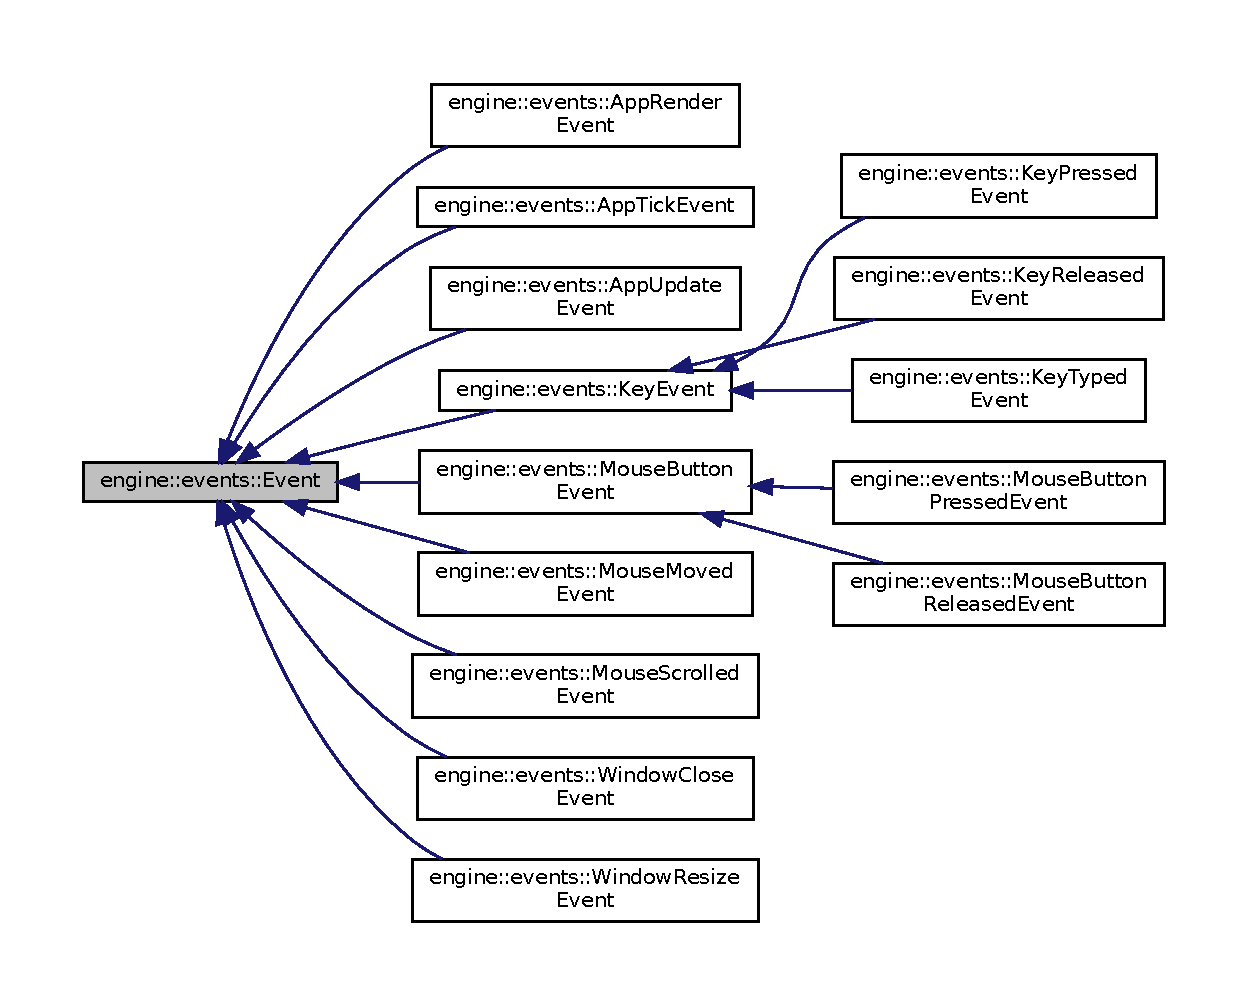
\includegraphics[width=350pt]{classengine_1_1events_1_1Event__inherit__graph}
\end{center}
\end{figure}
\subsection*{Public Member Functions}
\begin{DoxyCompactItemize}
\item 
\mbox{\Hypertarget{classengine_1_1events_1_1Event_a99604df0759386f2cea0071efa52d6e9}\label{classengine_1_1events_1_1Event_a99604df0759386f2cea0071efa52d6e9}} 
virtual \hyperlink{Event_8h_a10b3e1cfc8aaa02ff37fd47f0fae2b8a}{Event\+Type} {\bfseries Get\+Event\+Type} () const =0
\item 
\mbox{\Hypertarget{classengine_1_1events_1_1Event_a11bf339abb972f3c06f1cf20a0ff894b}\label{classengine_1_1events_1_1Event_a11bf339abb972f3c06f1cf20a0ff894b}} 
virtual const char $\ast$ {\bfseries Get\+Name} () const =0
\item 
\mbox{\Hypertarget{classengine_1_1events_1_1Event_a24e56efda02b259ac08ecc5ade26963d}\label{classengine_1_1events_1_1Event_a24e56efda02b259ac08ecc5ade26963d}} 
virtual int {\bfseries Get\+Category\+Flags} () const =0
\item 
\mbox{\Hypertarget{classengine_1_1events_1_1Event_afad3baa55387283c7cfe692292edc269}\label{classengine_1_1events_1_1Event_afad3baa55387283c7cfe692292edc269}} 
virtual std\+::string {\bfseries To\+String} () const
\item 
bool \hyperlink{classengine_1_1events_1_1Event_abf217454944fb4cceb6dee40d886a0c4}{Is\+In\+Category} (\hyperlink{Event_8h_a1e3bf91397b8a47069494aede2669474}{Event\+Category} category)
\begin{DoxyCompactList}\small\item\em Check if an event belongs to an Event\+Category. \end{DoxyCompactList}\item 
bool \hyperlink{classengine_1_1events_1_1Event_a8d8413f3ea8c3d00b3f43a757a92f623}{Has\+Been\+Handled} ()
\begin{DoxyCompactList}\small\item\em Check if an event has already been handled. \end{DoxyCompactList}\item 
\mbox{\Hypertarget{classengine_1_1events_1_1Event_aa3b39b29ab7c13070bc033bc88be4152}\label{classengine_1_1events_1_1Event_aa3b39b29ab7c13070bc033bc88be4152}} 
std\+::ostream \& \hyperlink{classengine_1_1events_1_1Event_aa3b39b29ab7c13070bc033bc88be4152}{operator$<$$<$} (std\+::ostream \&os)
\begin{DoxyCompactList}\small\item\em Allows events to be overloaded into. \end{DoxyCompactList}\end{DoxyCompactItemize}
\subsection*{Protected Member Functions}
\begin{DoxyCompactItemize}
\item 
\mbox{\Hypertarget{classengine_1_1events_1_1Event_aa85c36143880a3312b1c63166463ef5d}\label{classengine_1_1events_1_1Event_aa85c36143880a3312b1c63166463ef5d}} 
void {\bfseries Set\+Handled} (const bool success)
\end{DoxyCompactItemize}
\subsection*{Protected Attributes}
\begin{DoxyCompactItemize}
\item 
\mbox{\Hypertarget{classengine_1_1events_1_1Event_ad8e1eb6634225e11963228d6a69c166b}\label{classengine_1_1events_1_1Event_ad8e1eb6634225e11963228d6a69c166b}} 
bool {\bfseries has\+\_\+been\+\_\+handled\+\_\+} = false
\end{DoxyCompactItemize}
\subsection*{Friends}
\begin{DoxyCompactItemize}
\item 
\mbox{\Hypertarget{classengine_1_1events_1_1Event_aad5f38ccd490ea17008460423f52325a}\label{classengine_1_1events_1_1Event_aad5f38ccd490ea17008460423f52325a}} 
class {\bfseries Event\+Dispatcher}
\end{DoxyCompactItemize}


\subsection{Detailed Description}
The abstract \hyperlink{classengine_1_1events_1_1Event}{Event} class. 

The base \hyperlink{classengine_1_1events_1_1Event}{Event} implementation that is the parent class for any \hyperlink{classengine_1_1events_1_1Event}{Event} that would like to be passed into and handled by the \hyperlink{classengine_1_1events_1_1EventDispatcher}{Event\+Dispatcher} system. All Children class must override the functions provided by this class in order to be able to be propagated through the \hyperlink{classengine_1_1events_1_1EventDispatcher}{Event\+Dispatcher}. There are macros provided in {\ttfamily \hyperlink{Event_8h}{core/events/\+Event.\+h}} that are documented and make the process of creating child classes of \hyperlink{classengine_1_1events_1_1Event}{Event} magnitudes easier. 

\subsection{Member Function Documentation}
\mbox{\Hypertarget{classengine_1_1events_1_1Event_a8d8413f3ea8c3d00b3f43a757a92f623}\label{classengine_1_1events_1_1Event_a8d8413f3ea8c3d00b3f43a757a92f623}} 
\index{engine\+::events\+::\+Event@{engine\+::events\+::\+Event}!Has\+Been\+Handled@{Has\+Been\+Handled}}
\index{Has\+Been\+Handled@{Has\+Been\+Handled}!engine\+::events\+::\+Event@{engine\+::events\+::\+Event}}
\subsubsection{\texorpdfstring{Has\+Been\+Handled()}{HasBeenHandled()}}
{\footnotesize\ttfamily engine\+::events\+::\+Event\+::\+Has\+Been\+Handled (\begin{DoxyParamCaption}{ }\end{DoxyParamCaption})\hspace{0.3cm}{\ttfamily [inline]}}



Check if an event has already been handled. 

Only the \hyperlink{classengine_1_1events_1_1EventDispatcher}{Event\+Dispatcher} is capable of setting an event as being handled. \mbox{\Hypertarget{classengine_1_1events_1_1Event_abf217454944fb4cceb6dee40d886a0c4}\label{classengine_1_1events_1_1Event_abf217454944fb4cceb6dee40d886a0c4}} 
\index{engine\+::events\+::\+Event@{engine\+::events\+::\+Event}!Is\+In\+Category@{Is\+In\+Category}}
\index{Is\+In\+Category@{Is\+In\+Category}!engine\+::events\+::\+Event@{engine\+::events\+::\+Event}}
\subsubsection{\texorpdfstring{Is\+In\+Category()}{IsInCategory()}}
{\footnotesize\ttfamily engine\+::events\+::\+Event\+::\+Is\+In\+Category (\begin{DoxyParamCaption}\item[{\hyperlink{Event_8h_a1e3bf91397b8a47069494aede2669474}{Event\+Category}}]{category }\end{DoxyParamCaption})\hspace{0.3cm}{\ttfamily [inline]}}



Check if an event belongs to an Event\+Category. 


\begin{DoxyParams}{Parameters}
{\em category} & The category to be checked against. \\
\hline
\end{DoxyParams}


The documentation for this class was generated from the following file\+:\begin{DoxyCompactItemize}
\item 
engine/src/core/events/\hyperlink{Event_8h}{Event.\+h}\end{DoxyCompactItemize}

\hypertarget{classengine_1_1events_1_1EventDispatcher}{}\section{engine\+:\+:events\+:\+:Event\+Dispatcher Class Reference}
\label{classengine_1_1events_1_1EventDispatcher}\index{engine\+::events\+::\+Event\+Dispatcher@{engine\+::events\+::\+Event\+Dispatcher}}


{\ttfamily \#include $<$Event.\+h$>$}

\subsection*{Public Member Functions}
\begin{DoxyCompactItemize}
\item 
\mbox{\Hypertarget{classengine_1_1events_1_1EventDispatcher_a1a599ea2862fbf8ccff7510b3d1356f0}\label{classengine_1_1events_1_1EventDispatcher_a1a599ea2862fbf8ccff7510b3d1356f0}} 
{\bfseries Event\+Dispatcher} (\hyperlink{classengine_1_1events_1_1Event}{Event} $\ast$event)
\end{DoxyCompactItemize}


\subsection{Detailed Description}
The \hyperlink{classengine_1_1events_1_1EventDispatcher}{Event\+Dispatcher} is the key to handling all events. It is created per event and streamlines the process of dispatching events with callbacks that are invoked when the Event\+Type of the event used to create the \hyperlink{classengine_1_1events_1_1EventDispatcher}{Event\+Dispatcher} matches the Event\+Type that the callback is looking for. 

The documentation for this class was generated from the following file\+:\begin{DoxyCompactItemize}
\item 
engine/src/core/events/\hyperlink{Event_8h}{Event.\+h}\end{DoxyCompactItemize}

\hypertarget{classengine_1_1renderer_1_1GraphicsContext}{}\doxysection{engine\+::renderer\+::Graphics\+Context Class Reference}
\label{classengine_1_1renderer_1_1GraphicsContext}\index{engine::renderer::GraphicsContext@{engine::renderer::GraphicsContext}}


Inheritance diagram for engine\+::renderer\+::Graphics\+Context\+:
\nopagebreak
\begin{figure}[H]
\begin{center}
\leavevmode
\includegraphics[width=226pt]{classengine_1_1renderer_1_1GraphicsContext__inherit__graph}
\end{center}
\end{figure}
\doxysubsection*{Public Member Functions}
\begin{DoxyCompactItemize}
\item 
\mbox{\Hypertarget{classengine_1_1renderer_1_1GraphicsContext_ac7b94c5769b9464cdc2b71366fb0984b}\label{classengine_1_1renderer_1_1GraphicsContext_ac7b94c5769b9464cdc2b71366fb0984b}} 
virtual void {\bfseries Init} ()=0
\item 
\mbox{\Hypertarget{classengine_1_1renderer_1_1GraphicsContext_af4e7d29edd7912d32a07e139aef7a2f9}\label{classengine_1_1renderer_1_1GraphicsContext_af4e7d29edd7912d32a07e139aef7a2f9}} 
virtual void {\bfseries Swap\+Buffers} ()=0
\end{DoxyCompactItemize}


The documentation for this class was generated from the following file\+:\begin{DoxyCompactItemize}
\item 
engine/src/core/renderer/\mbox{\hyperlink{GraphicsContext_8h}{Graphics\+Context.\+h}}\end{DoxyCompactItemize}

\hypertarget{classengine_1_1imgui_1_1ImGuiLayer}{}\section{engine\+:\+:imgui\+:\+:Im\+Gui\+Layer Class Reference}
\label{classengine_1_1imgui_1_1ImGuiLayer}\index{engine\+::imgui\+::\+Im\+Gui\+Layer@{engine\+::imgui\+::\+Im\+Gui\+Layer}}


Inheritance diagram for engine\+:\+:imgui\+:\+:Im\+Gui\+Layer\+:
\nopagebreak
\begin{figure}[H]
\begin{center}
\leavevmode
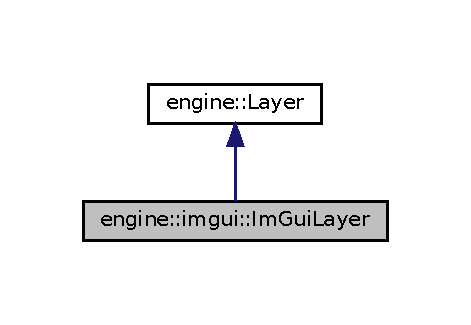
\includegraphics[width=211pt]{classengine_1_1imgui_1_1ImGuiLayer__inherit__graph}
\end{center}
\end{figure}


Collaboration diagram for engine\+:\+:imgui\+:\+:Im\+Gui\+Layer\+:
\nopagebreak
\begin{figure}[H]
\begin{center}
\leavevmode
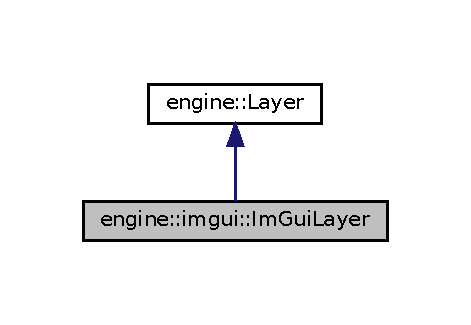
\includegraphics[width=211pt]{classengine_1_1imgui_1_1ImGuiLayer__coll__graph}
\end{center}
\end{figure}
\subsection*{Public Member Functions}
\begin{DoxyCompactItemize}
\item
\mbox{\Hypertarget{classengine_1_1imgui_1_1ImGuiLayer_ab3820ce44fcc9471f14c905510848f3e}\label{classengine_1_1imgui_1_1ImGuiLayer_ab3820ce44fcc9471f14c905510848f3e}}
void {\bfseries On\+Attach} () override
\item
\mbox{\Hypertarget{classengine_1_1imgui_1_1ImGuiLayer_af84a7c8e766167706345754587ced38e}\label{classengine_1_1imgui_1_1ImGuiLayer_af84a7c8e766167706345754587ced38e}}
void {\bfseries On\+Detach} () override
\item
\mbox{\Hypertarget{classengine_1_1imgui_1_1ImGuiLayer_aaa2388f874b2ede821ec8ba4f8642900}\label{classengine_1_1imgui_1_1ImGuiLayer_aaa2388f874b2ede821ec8ba4f8642900}}
void {\bfseries On\+Im\+Gui\+Render} () override
\item
\mbox{\Hypertarget{classengine_1_1imgui_1_1ImGuiLayer_a246081f496037b22475d76e3a9897ac9}\label{classengine_1_1imgui_1_1ImGuiLayer_a246081f496037b22475d76e3a9897ac9}}
void {\bfseries Begin} ()
\item
\mbox{\Hypertarget{classengine_1_1imgui_1_1ImGuiLayer_a7ad4c7169268bc19745b50b00282c9a9}\label{classengine_1_1imgui_1_1ImGuiLayer_a7ad4c7169268bc19745b50b00282c9a9}}
void {\bfseries End} ()
\end{DoxyCompactItemize}
\subsection*{Additional Inherited Members}


The documentation for this class was generated from the following files\+:\begin{DoxyCompactItemize}
\item
engine/src/core/imgui/Im\+Gui\+Layer.\+h\item
engine/src/core/imgui/Im\+Gui\+Layer.\+cpp\end{DoxyCompactItemize}

\hypertarget{classengine_1_1renderer_1_1IndexBuffer}{}\doxysection{engine\+::renderer\+::Index\+Buffer Class Reference}
\label{classengine_1_1renderer_1_1IndexBuffer}\index{engine::renderer::IndexBuffer@{engine::renderer::IndexBuffer}}


The base \mbox{\hyperlink{classengine_1_1renderer_1_1IndexBuffer}{Index\+Buffer}} class to be used for creating index buffers.  




{\ttfamily \#include $<$Buffer.\+h$>$}



Inheritance diagram for engine\+::renderer\+::Index\+Buffer\+:
% FIG 0
\doxysubsection*{Public Member Functions}
\begin{DoxyCompactItemize}
\item 
\mbox{\Hypertarget{classengine_1_1renderer_1_1IndexBuffer_a050664f22cc88b809bc386c1e4dba359}\label{classengine_1_1renderer_1_1IndexBuffer_a050664f22cc88b809bc386c1e4dba359}} 
virtual void \mbox{\hyperlink{classengine_1_1renderer_1_1IndexBuffer_a050664f22cc88b809bc386c1e4dba359}{Bind}} () const =0
\begin{DoxyCompactList}\small\item\em Bind the current \mbox{\hyperlink{classengine_1_1renderer_1_1IndexBuffer}{Index\+Buffer}} to the current rendering context. \end{DoxyCompactList}\item 
virtual void \mbox{\hyperlink{classengine_1_1renderer_1_1IndexBuffer_a8fd1ab43d3963533370c4d8e2e2282f4}{Unbind}} () const =0
\begin{DoxyCompactList}\small\item\em Unbind the current \mbox{\hyperlink{classengine_1_1renderer_1_1IndexBuffer}{Index\+Buffer}} from the current rendering context. \end{DoxyCompactList}\item 
\mbox{\Hypertarget{classengine_1_1renderer_1_1IndexBuffer_a42571fcc830427648852258124e92844}\label{classengine_1_1renderer_1_1IndexBuffer_a42571fcc830427648852258124e92844}} 
virtual uint32\+\_\+t \mbox{\hyperlink{classengine_1_1renderer_1_1IndexBuffer_a42571fcc830427648852258124e92844}{Get\+Count}} () const =0
\begin{DoxyCompactList}\small\item\em Get the count of indices within the current \mbox{\hyperlink{classengine_1_1renderer_1_1IndexBuffer}{Index\+Buffer}}. \end{DoxyCompactList}\end{DoxyCompactItemize}
\doxysubsection*{Static Public Member Functions}
\begin{DoxyCompactItemize}
\item 
static memory\+::\+Shared$<$ \mbox{\hyperlink{classengine_1_1renderer_1_1IndexBuffer}{Index\+Buffer}} $>$ \mbox{\hyperlink{classengine_1_1renderer_1_1IndexBuffer_a2a4773cdd0dab8101ca9662ff6c0a460}{Create}} (uint32\+\_\+t $\ast$indices, uint32\+\_\+t count)
\begin{DoxyCompactList}\small\item\em Creates a \mbox{\hyperlink{classengine_1_1renderer_1_1IndexBuffer}{Index\+Buffer}} through the Graphics A\+PI that is being used at compile time. \end{DoxyCompactList}\end{DoxyCompactItemize}


\doxysubsection{Detailed Description}
The base \mbox{\hyperlink{classengine_1_1renderer_1_1IndexBuffer}{Index\+Buffer}} class to be used for creating index buffers. 

Platform specific graphics A\+PI should extend this class in order to be supported by the the rendering A\+PI. 

\doxysubsection{Member Function Documentation}
\mbox{\Hypertarget{classengine_1_1renderer_1_1IndexBuffer_a2a4773cdd0dab8101ca9662ff6c0a460}\label{classengine_1_1renderer_1_1IndexBuffer_a2a4773cdd0dab8101ca9662ff6c0a460}} 
\index{engine::renderer::IndexBuffer@{engine::renderer::IndexBuffer}!Create@{Create}}
\index{Create@{Create}!engine::renderer::IndexBuffer@{engine::renderer::IndexBuffer}}
\doxysubsubsection{\texorpdfstring{Create()}{Create()}}
{\footnotesize\ttfamily engine\+::renderer\+::\+Index\+Buffer\+::\+Create (\begin{DoxyParamCaption}\item[{uint32\+\_\+t $\ast$}]{indices,  }\item[{uint32\+\_\+t}]{count }\end{DoxyParamCaption})\hspace{0.3cm}{\ttfamily [static]}}



Creates a \mbox{\hyperlink{classengine_1_1renderer_1_1IndexBuffer}{Index\+Buffer}} through the Graphics A\+PI that is being used at compile time. 


\begin{DoxyParams}{Parameters}
{\em indices} & -\/ a pointer to an array of indices to be registered. \\
\hline
{\em size} & -\/ The size of the vertices in bytes. This is the primary method of creating platform independent index buffers and what should be used by users to create Vertex Buffers that are compatible with the rendering A\+PI. \\
\hline
\end{DoxyParams}
\mbox{\Hypertarget{classengine_1_1renderer_1_1IndexBuffer_a8fd1ab43d3963533370c4d8e2e2282f4}\label{classengine_1_1renderer_1_1IndexBuffer_a8fd1ab43d3963533370c4d8e2e2282f4}} 
\index{engine::renderer::IndexBuffer@{engine::renderer::IndexBuffer}!Unbind@{Unbind}}
\index{Unbind@{Unbind}!engine::renderer::IndexBuffer@{engine::renderer::IndexBuffer}}
\doxysubsubsection{\texorpdfstring{Unbind()}{Unbind()}}
{\footnotesize\ttfamily engine\+::renderer\+::\+Index\+Buffer\+::\+Unbind (\begin{DoxyParamCaption}{ }\end{DoxyParamCaption}) const\hspace{0.3cm}{\ttfamily [pure virtual]}}



Unbind the current \mbox{\hyperlink{classengine_1_1renderer_1_1IndexBuffer}{Index\+Buffer}} from the current rendering context. 

Any vertex buffer that relies on this buffer will not be able to access the contents of it once unbound from the graphics context. 

Implemented in \mbox{\hyperlink{classengine_1_1platform_1_1opengl_1_1OpenGLIndexBuffer_a9fc400e4c464a2dbf7df76eba359639e}{engine\+::platform\+::opengl\+::\+Open\+G\+L\+Index\+Buffer}}.



The documentation for this class was generated from the following files\+:\begin{DoxyCompactItemize}
\item 
engine/src/core/renderer/\mbox{\hyperlink{Buffer_8h}{Buffer.\+h}}\item 
engine/src/core/renderer/Buffer.\+cpp\end{DoxyCompactItemize}

\hypertarget{classengine_1_1Input}{}\section{engine\+:\+:Input Class Reference}
\label{classengine_1_1Input}\index{engine\+::\+Input@{engine\+::\+Input}}
\subsection*{Static Public Member Functions}
\begin{DoxyCompactItemize}
\item 
\mbox{\Hypertarget{classengine_1_1Input_a79ec265ab6800cb0b1f627bfdb3cfc28}\label{classengine_1_1Input_a79ec265ab6800cb0b1f627bfdb3cfc28}} 
static bool {\bfseries Is\+Key\+Pressed} (int key\+\_\+code)
\item 
\mbox{\Hypertarget{classengine_1_1Input_a13095584400184088868e6ff9c9f0a5d}\label{classengine_1_1Input_a13095584400184088868e6ff9c9f0a5d}} 
static float {\bfseries Get\+MouseX} ()
\item 
\mbox{\Hypertarget{classengine_1_1Input_aa6fa67ccfdb48ac903c927157f0809c2}\label{classengine_1_1Input_aa6fa67ccfdb48ac903c927157f0809c2}} 
static float {\bfseries Get\+MouseY} ()
\item 
\mbox{\Hypertarget{classengine_1_1Input_a4a15d91ac4241fc6dc3584c051e1b50a}\label{classengine_1_1Input_a4a15d91ac4241fc6dc3584c051e1b50a}} 
static std\+::pair$<$ float, float $>$ {\bfseries Get\+Mouse\+Position} ()
\item 
\mbox{\Hypertarget{classengine_1_1Input_acaa32590a2b39e0eb822c01d5b7815dc}\label{classengine_1_1Input_acaa32590a2b39e0eb822c01d5b7815dc}} 
static bool {\bfseries Is\+Mouse\+Button\+Pressed} (int button)
\end{DoxyCompactItemize}
\subsection*{Protected Member Functions}
\begin{DoxyCompactItemize}
\item 
\mbox{\Hypertarget{classengine_1_1Input_a296cc17bac6e2ebc45d178c3c06c0d63}\label{classengine_1_1Input_a296cc17bac6e2ebc45d178c3c06c0d63}} 
virtual bool {\bfseries Is\+Key\+Pressed\+Impl} (int key\+\_\+code)=0
\item 
\mbox{\Hypertarget{classengine_1_1Input_ad9b92c2cccac4db3431bed2143326329}\label{classengine_1_1Input_ad9b92c2cccac4db3431bed2143326329}} 
virtual float {\bfseries Get\+Mouse\+X\+Impl} ()=0
\item 
\mbox{\Hypertarget{classengine_1_1Input_a490d05f204808bdae219da6d1b03eb12}\label{classengine_1_1Input_a490d05f204808bdae219da6d1b03eb12}} 
virtual float {\bfseries Get\+Mouse\+Y\+Impl} ()=0
\item 
\mbox{\Hypertarget{classengine_1_1Input_a0d98b07560fa833c7a482341e6c76dbc}\label{classengine_1_1Input_a0d98b07560fa833c7a482341e6c76dbc}} 
virtual std\+::pair$<$ float, float $>$ {\bfseries Get\+Mouse\+Position\+Impl} ()=0
\item 
\mbox{\Hypertarget{classengine_1_1Input_a9fb17f21b15540890cb69d87d3749cdd}\label{classengine_1_1Input_a9fb17f21b15540890cb69d87d3749cdd}} 
virtual bool {\bfseries Is\+Mouse\+Button\+Pressed\+Impl} (int button)=0
\end{DoxyCompactItemize}


The documentation for this class was generated from the following file\+:\begin{DoxyCompactItemize}
\item 
engine/src/core/Input.\+h\end{DoxyCompactItemize}

\hypertarget{classengine_1_1events_1_1KeyEvent}{}\section{engine\+:\+:events\+:\+:Key\+Event Class Reference}
\label{classengine_1_1events_1_1KeyEvent}\index{engine\+::events\+::\+Key\+Event@{engine\+::events\+::\+Key\+Event}}


The base event for all other Key input events.  




{\ttfamily \#include $<$Key\+Event.\+h$>$}



Inheritance diagram for engine\+:\+:events\+:\+:Key\+Event\+:\nopagebreak
\begin{figure}[H]
\begin{center}
\leavevmode
\includegraphics[width=350pt]{classengine_1_1events_1_1KeyEvent__inherit__graph}
\end{center}
\end{figure}


Collaboration diagram for engine\+:\+:events\+:\+:Key\+Event\+:\nopagebreak
\begin{figure}[H]
\begin{center}
\leavevmode
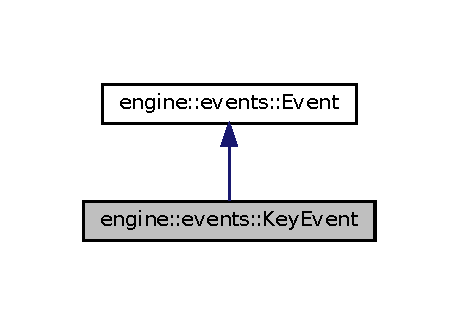
\includegraphics[width=209pt]{classengine_1_1events_1_1KeyEvent__coll__graph}
\end{center}
\end{figure}
\subsection*{Public Member Functions}
\begin{DoxyCompactItemize}
\item 
int \hyperlink{classengine_1_1events_1_1KeyEvent_a2140c6615ec67c2f0cca0b1932968947}{Get\+Key\+Code} () const
\begin{DoxyCompactList}\small\item\em obtain the key code that generated the user had input into the application. \end{DoxyCompactList}\end{DoxyCompactItemize}
\subsection*{Protected Member Functions}
\begin{DoxyCompactItemize}
\item 
\mbox{\Hypertarget{classengine_1_1events_1_1KeyEvent_a621562a39051187801b6f7259542a04f}\label{classengine_1_1events_1_1KeyEvent_a621562a39051187801b6f7259542a04f}} 
\hyperlink{classengine_1_1events_1_1KeyEvent_a621562a39051187801b6f7259542a04f}{Key\+Event} (int key\+\_\+code)
\begin{DoxyCompactList}\small\item\em Only classes that derive from the \hyperlink{classengine_1_1events_1_1KeyEvent}{Key\+Event} class are allowed to invoke the constructor of the \hyperlink{classengine_1_1events_1_1KeyEvent}{Key\+Event} class. \end{DoxyCompactList}\end{DoxyCompactItemize}
\subsection*{Protected Attributes}
\begin{DoxyCompactItemize}
\item 
\mbox{\Hypertarget{classengine_1_1events_1_1KeyEvent_addcbfb73fa603f77369b613d87d76875}\label{classengine_1_1events_1_1KeyEvent_addcbfb73fa603f77369b613d87d76875}} 
int {\bfseries key\+\_\+code\+\_\+}
\end{DoxyCompactItemize}


\subsection{Detailed Description}
The base event for all other Key input events. 

Registers the \hyperlink{classengine_1_1events_1_1Event}{Event} category as both a keyboard and input event. (See Event\+Category for more types of event categories) 

\subsection{Member Function Documentation}
\mbox{\Hypertarget{classengine_1_1events_1_1KeyEvent_a2140c6615ec67c2f0cca0b1932968947}\label{classengine_1_1events_1_1KeyEvent_a2140c6615ec67c2f0cca0b1932968947}} 
\index{engine\+::events\+::\+Key\+Event@{engine\+::events\+::\+Key\+Event}!Get\+Key\+Code@{Get\+Key\+Code}}
\index{Get\+Key\+Code@{Get\+Key\+Code}!engine\+::events\+::\+Key\+Event@{engine\+::events\+::\+Key\+Event}}
\subsubsection{\texorpdfstring{Get\+Key\+Code()}{GetKeyCode()}}
{\footnotesize\ttfamily engine\+::events\+::\+Key\+Event\+::\+Get\+Key\+Code (\begin{DoxyParamCaption}{ }\end{DoxyParamCaption}) const\hspace{0.3cm}{\ttfamily [inline]}}



obtain the key code that generated the user had input into the application. 

This should reference engine key codes, and not any platform specific ones. 

The documentation for this class was generated from the following file\+:\begin{DoxyCompactItemize}
\item 
engine/src/core/events/\hyperlink{KeyEvent_8h}{Key\+Event.\+h}\end{DoxyCompactItemize}

\hypertarget{classengine_1_1events_1_1KeyPressedEvent}{}\section{engine\+:\+:events\+:\+:Key\+Pressed\+Event Class Reference}
\label{classengine_1_1events_1_1KeyPressedEvent}\index{engine\+::events\+::\+Key\+Pressed\+Event@{engine\+::events\+::\+Key\+Pressed\+Event}}


Inheritance diagram for engine\+:\+:events\+:\+:Key\+Pressed\+Event\+:
\nopagebreak
\begin{figure}[H]
\begin{center}
\leavevmode
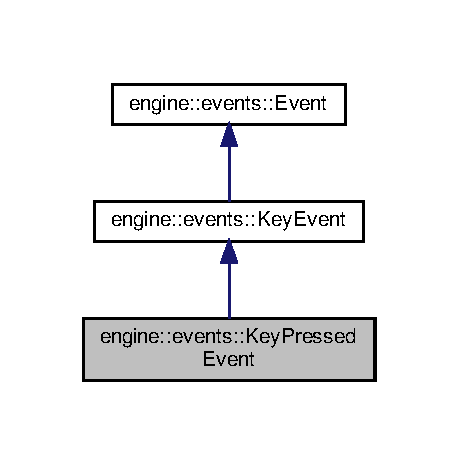
\includegraphics[width=220pt]{classengine_1_1events_1_1KeyPressedEvent__inherit__graph}
\end{center}
\end{figure}


Collaboration diagram for engine\+:\+:events\+:\+:Key\+Pressed\+Event\+:
\nopagebreak
\begin{figure}[H]
\begin{center}
\leavevmode
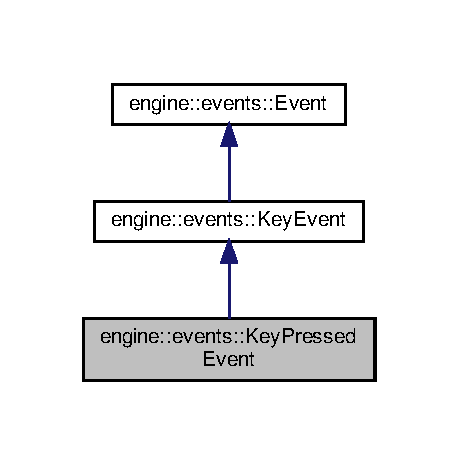
\includegraphics[width=220pt]{classengine_1_1events_1_1KeyPressedEvent__coll__graph}
\end{center}
\end{figure}
\subsection*{Public Member Functions}
\begin{DoxyCompactItemize}
\item
\mbox{\Hypertarget{classengine_1_1events_1_1KeyPressedEvent_adc492a01f4883f3632a30042891bc97a}\label{classengine_1_1events_1_1KeyPressedEvent_adc492a01f4883f3632a30042891bc97a}}
{\bfseries Key\+Pressed\+Event} (int key\+\_\+code, int repeat\+\_\+count)
\item
\mbox{\Hypertarget{classengine_1_1events_1_1KeyPressedEvent_a3ad3835c19b60dee03e9cd819f9a43ff}\label{classengine_1_1events_1_1KeyPressedEvent_a3ad3835c19b60dee03e9cd819f9a43ff}}
int {\bfseries Get\+Repeat\+Count} () const
\item
\mbox{\Hypertarget{classengine_1_1events_1_1KeyPressedEvent_af7c728af6e5a62418cb1faee0710e9ad}\label{classengine_1_1events_1_1KeyPressedEvent_af7c728af6e5a62418cb1faee0710e9ad}}
std\+::string {\bfseries To\+String} () const override
\item
\mbox{\Hypertarget{classengine_1_1events_1_1KeyPressedEvent_a67a1b66f53a5ec23d70c374a64530056}\label{classengine_1_1events_1_1KeyPressedEvent_a67a1b66f53a5ec23d70c374a64530056}}
{\bfseries E\+V\+E\+N\+T\+\_\+\+C\+L\+A\+S\+S\+\_\+\+T\+Y\+PE} (k\+Key\+Pressed)
\end{DoxyCompactItemize}
\subsection*{Additional Inherited Members}


The documentation for this class was generated from the following file\+:\begin{DoxyCompactItemize}
\item
engine/src/core/events/Key\+Event.\+h\end{DoxyCompactItemize}

\hypertarget{classengine_1_1events_1_1KeyReleasedEvent}{}\section{engine\+:\+:events\+:\+:Key\+Released\+Event Class Reference}
\label{classengine_1_1events_1_1KeyReleasedEvent}\index{engine\+::events\+::\+Key\+Released\+Event@{engine\+::events\+::\+Key\+Released\+Event}}


Inheritance diagram for engine\+:\+:events\+:\+:Key\+Released\+Event\+:
\nopagebreak
\begin{figure}[H]
\begin{center}
\leavevmode
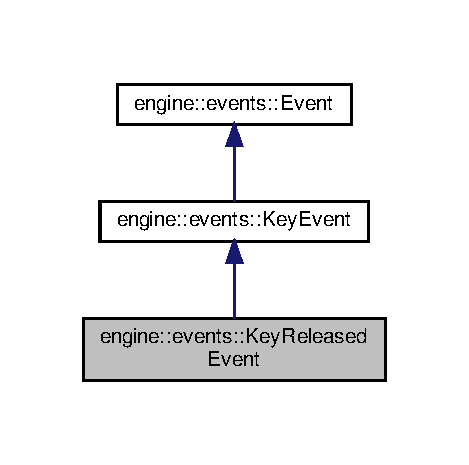
\includegraphics[width=225pt]{classengine_1_1events_1_1KeyReleasedEvent__inherit__graph}
\end{center}
\end{figure}


Collaboration diagram for engine\+:\+:events\+:\+:Key\+Released\+Event\+:
\nopagebreak
\begin{figure}[H]
\begin{center}
\leavevmode
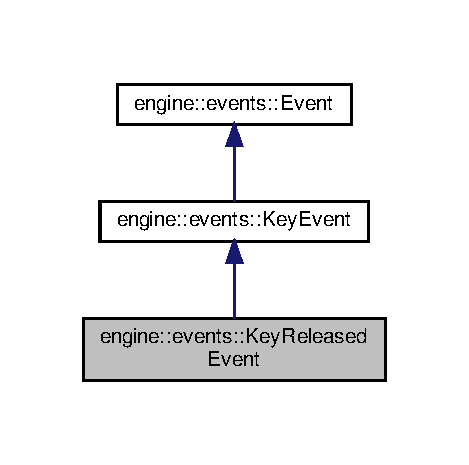
\includegraphics[width=225pt]{classengine_1_1events_1_1KeyReleasedEvent__coll__graph}
\end{center}
\end{figure}
\subsection*{Public Member Functions}
\begin{DoxyCompactItemize}
\item
\mbox{\Hypertarget{classengine_1_1events_1_1KeyReleasedEvent_a6e5c52cc5adcfa7f9afd36557125b1d5}\label{classengine_1_1events_1_1KeyReleasedEvent_a6e5c52cc5adcfa7f9afd36557125b1d5}}
{\bfseries Key\+Released\+Event} (int key\+\_\+code)
\item
\mbox{\Hypertarget{classengine_1_1events_1_1KeyReleasedEvent_a7b7e3848f31974623a24708aafdc9d69}\label{classengine_1_1events_1_1KeyReleasedEvent_a7b7e3848f31974623a24708aafdc9d69}}
std\+::string {\bfseries To\+String} () const override
\end{DoxyCompactItemize}
\subsection*{Additional Inherited Members}


The documentation for this class was generated from the following file\+:\begin{DoxyCompactItemize}
\item
engine/src/core/events/Key\+Event.\+h\end{DoxyCompactItemize}

\hypertarget{classengine_1_1events_1_1KeyTypedEvent}{}\section{engine\+:\+:events\+:\+:Key\+Typed\+Event Class Reference}
\label{classengine_1_1events_1_1KeyTypedEvent}\index{engine\+::events\+::\+Key\+Typed\+Event@{engine\+::events\+::\+Key\+Typed\+Event}}


Inheritance diagram for engine\+:\+:events\+:\+:Key\+Typed\+Event\+:
\nopagebreak
\begin{figure}[H]
\begin{center}
\leavevmode
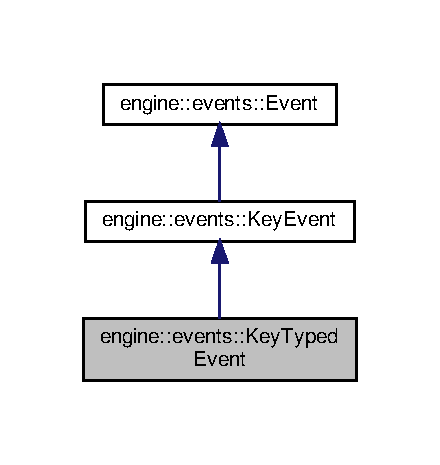
\includegraphics[width=211pt]{classengine_1_1events_1_1KeyTypedEvent__inherit__graph}
\end{center}
\end{figure}


Collaboration diagram for engine\+:\+:events\+:\+:Key\+Typed\+Event\+:
\nopagebreak
\begin{figure}[H]
\begin{center}
\leavevmode
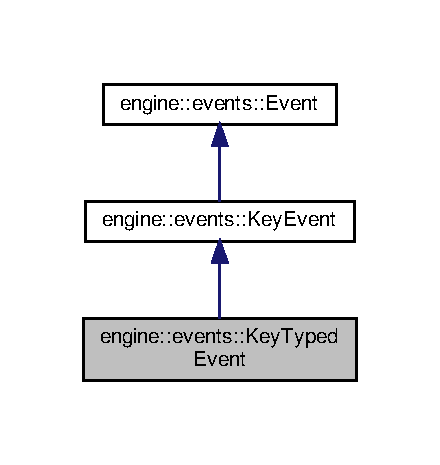
\includegraphics[width=211pt]{classengine_1_1events_1_1KeyTypedEvent__coll__graph}
\end{center}
\end{figure}
\subsection*{Public Member Functions}
\begin{DoxyCompactItemize}
\item 
\mbox{\Hypertarget{classengine_1_1events_1_1KeyTypedEvent_a8e73360c78c5abefc838c7cbea09213f}\label{classengine_1_1events_1_1KeyTypedEvent_a8e73360c78c5abefc838c7cbea09213f}} 
{\bfseries Key\+Typed\+Event} (int key\+\_\+code)
\item 
\mbox{\Hypertarget{classengine_1_1events_1_1KeyTypedEvent_af805e57bdf4ae3df824a73d1465a603e}\label{classengine_1_1events_1_1KeyTypedEvent_af805e57bdf4ae3df824a73d1465a603e}} 
std\+::string {\bfseries To\+String} () const override
\item 
\mbox{\Hypertarget{classengine_1_1events_1_1KeyTypedEvent_a1973d84e5946e3c52a293b5faf128409}\label{classengine_1_1events_1_1KeyTypedEvent_a1973d84e5946e3c52a293b5faf128409}} 
{\bfseries E\+V\+E\+N\+T\+\_\+\+C\+L\+A\+S\+S\+\_\+\+T\+Y\+PE} (k\+Key\+Typed)
\end{DoxyCompactItemize}
\subsection*{Additional Inherited Members}


The documentation for this class was generated from the following file\+:\begin{DoxyCompactItemize}
\item 
engine/src/core/events/Key\+Event.\+h\end{DoxyCompactItemize}

\hypertarget{classengine_1_1Layer}{}\doxysection{engine\+::Layer Class Reference}
\label{classengine_1_1Layer}\index{engine::Layer@{engine::Layer}}


Inheritance diagram for engine\+::Layer\+:\nopagebreak
\begin{figure}[H]
\begin{center}
\leavevmode
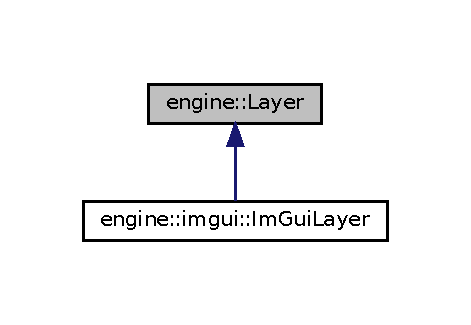
\includegraphics[width=226pt]{classengine_1_1Layer__inherit__graph}
\end{center}
\end{figure}
\doxysubsection*{Public Member Functions}
\begin{DoxyCompactItemize}
\item 
\mbox{\Hypertarget{classengine_1_1Layer_a7c94872b9fc69fd1695e21319c6ae495}\label{classengine_1_1Layer_a7c94872b9fc69fd1695e21319c6ae495}} 
{\bfseries Layer} (const std\+::string \&name=\char`\"{}Layer\char`\"{})
\item 
virtual void \mbox{\hyperlink{classengine_1_1Layer_ace68c1d4e441165d6741a74d4b11c7f0}{On\+Attach}} ()
\begin{DoxyCompactList}\small\item\em What to do when a layer is attached to the game engine. \end{DoxyCompactList}\item 
virtual void \mbox{\hyperlink{classengine_1_1Layer_acfa7e624cfd2cb85803382511454d098}{On\+Detach}} ()
\begin{DoxyCompactList}\small\item\em Handles what to do when a layer is attached to the game engine. \end{DoxyCompactList}\item 
virtual void \mbox{\hyperlink{classengine_1_1Layer_a85ce49ee4b9f58cad1b302c3cb4a8207}{On\+Update}} (\mbox{\hyperlink{classengine_1_1util_1_1TimeStep}{util\+::\+Time\+Step}} time\+\_\+step)
\begin{DoxyCompactList}\small\item\em Handles what to do when the game engine requests to update the layer. \end{DoxyCompactList}\item 
virtual void \mbox{\hyperlink{classengine_1_1Layer_a982be4dc6ab1d3d71162719138312872}{On\+Event}} (\mbox{\hyperlink{classengine_1_1events_1_1Event}{events\+::\+Event}} $\ast$event)
\begin{DoxyCompactList}\small\item\em Handles what to do when the game engine passes an event. \end{DoxyCompactList}\item 
virtual void \mbox{\hyperlink{classengine_1_1Layer_a002df9fddaba135a8bd7abc14e3fb067}{On\+Im\+Gui\+Render}} ()
\begin{DoxyCompactList}\small\item\em Handles what to do when the game engine requests the layer to render Im\+Gui components. \end{DoxyCompactList}\item 
const std\+::string \& \mbox{\hyperlink{classengine_1_1Layer_a770a8fb58326ed32779e84bf54a93eef}{Get\+Name}} () const
\begin{DoxyCompactList}\small\item\em Gets the name of the layer. \end{DoxyCompactList}\end{DoxyCompactItemize}
\doxysubsection*{Protected Attributes}
\begin{DoxyCompactItemize}
\item 
\mbox{\Hypertarget{classengine_1_1Layer_a9283719bf3b3d956809ef351a43ee16f}\label{classengine_1_1Layer_a9283719bf3b3d956809ef351a43ee16f}} 
std\+::string {\bfseries debug\+\_\+name\+\_\+}
\end{DoxyCompactItemize}


\doxysubsection{Member Function Documentation}
\mbox{\Hypertarget{classengine_1_1Layer_a770a8fb58326ed32779e84bf54a93eef}\label{classengine_1_1Layer_a770a8fb58326ed32779e84bf54a93eef}} 
\index{engine::Layer@{engine::Layer}!GetName@{GetName}}
\index{GetName@{GetName}!engine::Layer@{engine::Layer}}
\doxysubsubsection{\texorpdfstring{GetName()}{GetName()}}
{\footnotesize\ttfamily engine\+::\+Layer\+::\+Get\+Name (\begin{DoxyParamCaption}{ }\end{DoxyParamCaption}) const\hspace{0.3cm}{\ttfamily [inline]}}



Gets the name of the layer. 

Mainly used for debugging within the engine. \mbox{\Hypertarget{classengine_1_1Layer_ace68c1d4e441165d6741a74d4b11c7f0}\label{classengine_1_1Layer_ace68c1d4e441165d6741a74d4b11c7f0}} 
\index{engine::Layer@{engine::Layer}!OnAttach@{OnAttach}}
\index{OnAttach@{OnAttach}!engine::Layer@{engine::Layer}}
\doxysubsubsection{\texorpdfstring{OnAttach()}{OnAttach()}}
{\footnotesize\ttfamily engine\+::\+Layer\+::\+On\+Attach (\begin{DoxyParamCaption}{ }\end{DoxyParamCaption})\hspace{0.3cm}{\ttfamily [inline]}, {\ttfamily [virtual]}}



What to do when a layer is attached to the game engine. 

Primarily for initializing anything in the layer when it\textquotesingle{}s attached to the engine. 

Reimplemented in \mbox{\hyperlink{classengine_1_1imgui_1_1ImGuiLayer_a8580bd31942d4bc33f268053d2adec31}{engine\+::imgui\+::\+Im\+Gui\+Layer}}.

\mbox{\Hypertarget{classengine_1_1Layer_acfa7e624cfd2cb85803382511454d098}\label{classengine_1_1Layer_acfa7e624cfd2cb85803382511454d098}} 
\index{engine::Layer@{engine::Layer}!OnDetach@{OnDetach}}
\index{OnDetach@{OnDetach}!engine::Layer@{engine::Layer}}
\doxysubsubsection{\texorpdfstring{OnDetach()}{OnDetach()}}
{\footnotesize\ttfamily engine\+::\+Layer\+::\+On\+Detach (\begin{DoxyParamCaption}{ }\end{DoxyParamCaption})\hspace{0.3cm}{\ttfamily [inline]}, {\ttfamily [virtual]}}



Handles what to do when a layer is attached to the game engine. 

Primarily for cleaning up anything in the layer when it\textquotesingle{}s no longer attached to the engine. 

Reimplemented in \mbox{\hyperlink{classengine_1_1imgui_1_1ImGuiLayer_ad443a984abe93f4101fdbadcea01bf9b}{engine\+::imgui\+::\+Im\+Gui\+Layer}}.

\mbox{\Hypertarget{classengine_1_1Layer_a982be4dc6ab1d3d71162719138312872}\label{classengine_1_1Layer_a982be4dc6ab1d3d71162719138312872}} 
\index{engine::Layer@{engine::Layer}!OnEvent@{OnEvent}}
\index{OnEvent@{OnEvent}!engine::Layer@{engine::Layer}}
\doxysubsubsection{\texorpdfstring{OnEvent()}{OnEvent()}}
{\footnotesize\ttfamily engine\+::\+Layer\+::\+On\+Event (\begin{DoxyParamCaption}\item[{\mbox{\hyperlink{classengine_1_1events_1_1Event}{events\+::\+Event}} $\ast$}]{event }\end{DoxyParamCaption})\hspace{0.3cm}{\ttfamily [inline]}, {\ttfamily [virtual]}}



Handles what to do when the game engine passes an event. 


\begin{DoxyParams}{Parameters}
{\em event} & -\/ The event received by the engine. This can only be accessed if the layer is attached to the engine. \\
\hline
\end{DoxyParams}
\mbox{\Hypertarget{classengine_1_1Layer_a002df9fddaba135a8bd7abc14e3fb067}\label{classengine_1_1Layer_a002df9fddaba135a8bd7abc14e3fb067}} 
\index{engine::Layer@{engine::Layer}!OnImGuiRender@{OnImGuiRender}}
\index{OnImGuiRender@{OnImGuiRender}!engine::Layer@{engine::Layer}}
\doxysubsubsection{\texorpdfstring{OnImGuiRender()}{OnImGuiRender()}}
{\footnotesize\ttfamily engine\+::\+Layer\+::\+On\+Im\+Gui\+Render (\begin{DoxyParamCaption}{ }\end{DoxyParamCaption})\hspace{0.3cm}{\ttfamily [inline]}, {\ttfamily [virtual]}}



Handles what to do when the game engine requests the layer to render Im\+Gui components. 

This can only be accessed if the layer is attached to the engine. 

Reimplemented in \mbox{\hyperlink{classengine_1_1imgui_1_1ImGuiLayer_aeacc4aecfc119192fbe98e961b88813e}{engine\+::imgui\+::\+Im\+Gui\+Layer}}.

\mbox{\Hypertarget{classengine_1_1Layer_a85ce49ee4b9f58cad1b302c3cb4a8207}\label{classengine_1_1Layer_a85ce49ee4b9f58cad1b302c3cb4a8207}} 
\index{engine::Layer@{engine::Layer}!OnUpdate@{OnUpdate}}
\index{OnUpdate@{OnUpdate}!engine::Layer@{engine::Layer}}
\doxysubsubsection{\texorpdfstring{OnUpdate()}{OnUpdate()}}
{\footnotesize\ttfamily engine\+::\+Layer\+::\+On\+Update (\begin{DoxyParamCaption}\item[{\mbox{\hyperlink{classengine_1_1util_1_1TimeStep}{util\+::\+Time\+Step}}}]{time\+\_\+step }\end{DoxyParamCaption})\hspace{0.3cm}{\ttfamily [inline]}, {\ttfamily [virtual]}}



Handles what to do when the game engine requests to update the layer. 

This can only be accessed if the layer is attached to the engine. 

The documentation for this class was generated from the following files\+:\begin{DoxyCompactItemize}
\item 
engine/src/core/\mbox{\hyperlink{Layer_8h}{Layer.\+h}}\item 
engine/src/core/Layer.\+cpp\end{DoxyCompactItemize}

\hypertarget{classengine_1_1LayerStack}{}\section{engine\+:\+:Layer\+Stack Class Reference}
\label{classengine_1_1LayerStack}\index{engine\+::\+Layer\+Stack@{engine\+::\+Layer\+Stack}}
\subsection*{Public Member Functions}
\begin{DoxyCompactItemize}
\item 
\mbox{\Hypertarget{classengine_1_1LayerStack_a3e18dd7877bf00498b9771cf91fc9b7c}\label{classengine_1_1LayerStack_a3e18dd7877bf00498b9771cf91fc9b7c}} 
void {\bfseries Push\+Layer} (\hyperlink{classengine_1_1Layer}{Layer} $\ast$layer)
\item 
\mbox{\Hypertarget{classengine_1_1LayerStack_a4b84a2581e5647cd73b5924c7982680f}\label{classengine_1_1LayerStack_a4b84a2581e5647cd73b5924c7982680f}} 
void {\bfseries Push\+Overlay} (\hyperlink{classengine_1_1Layer}{Layer} $\ast$overlay)
\item 
\mbox{\Hypertarget{classengine_1_1LayerStack_a864050f5ad6ed9ffe04974c9411fad94}\label{classengine_1_1LayerStack_a864050f5ad6ed9ffe04974c9411fad94}} 
void {\bfseries Pop\+Layer} (\hyperlink{classengine_1_1Layer}{Layer} $\ast$layer)
\item 
\mbox{\Hypertarget{classengine_1_1LayerStack_aecbddf93a6f5846a902570a980a63ddb}\label{classengine_1_1LayerStack_aecbddf93a6f5846a902570a980a63ddb}} 
void {\bfseries Pop\+Overlay} (\hyperlink{classengine_1_1Layer}{Layer} $\ast$layer)
\item 
\mbox{\Hypertarget{classengine_1_1LayerStack_a341bf522aa1af78ba06e3fdf510df271}\label{classengine_1_1LayerStack_a341bf522aa1af78ba06e3fdf510df271}} 
std\+::vector$<$ \hyperlink{classengine_1_1Layer}{Layer} $\ast$ $>$\+::iterator {\bfseries begin} ()
\item 
\mbox{\Hypertarget{classengine_1_1LayerStack_ad05cf0f1deec9dd7f7d8ead15febf657}\label{classengine_1_1LayerStack_ad05cf0f1deec9dd7f7d8ead15febf657}} 
std\+::vector$<$ \hyperlink{classengine_1_1Layer}{Layer} $\ast$ $>$\+::iterator {\bfseries end} ()
\end{DoxyCompactItemize}


The documentation for this class was generated from the following files\+:\begin{DoxyCompactItemize}
\item 
engine/src/core/Layer\+Stack.\+h\item 
engine/src/core/Layer\+Stack.\+cpp\end{DoxyCompactItemize}

\hypertarget{classengine_1_1logging_1_1Log}{}\doxysection{engine\+::logging\+::Log Class Reference}
\label{classengine_1_1logging_1_1Log}\index{engine::logging::Log@{engine::logging::Log}}


The container class for managing static instances of the engine and client loggers.  




{\ttfamily \#include $<$Log.\+h$>$}

\doxysubsection*{Static Public Member Functions}
\begin{DoxyCompactItemize}
\item 
\mbox{\Hypertarget{classengine_1_1logging_1_1Log_a1364bca4f007e2931a0110f91e3e13c4}\label{classengine_1_1logging_1_1Log_a1364bca4f007e2931a0110f91e3e13c4}} 
static void {\bfseries Init} ()
\item 
\mbox{\Hypertarget{classengine_1_1logging_1_1Log_ad54813613a17e01d3272b9fb124b049e}\label{classengine_1_1logging_1_1Log_ad54813613a17e01d3272b9fb124b049e}} 
static std\+::shared\+\_\+ptr$<$ spdlog\+::logger $>$ \& {\bfseries Get\+Core\+Logger} ()
\item 
\mbox{\Hypertarget{classengine_1_1logging_1_1Log_abae59faa07a4ce0d627772e79073c67b}\label{classengine_1_1logging_1_1Log_abae59faa07a4ce0d627772e79073c67b}} 
static std\+::shared\+\_\+ptr$<$ spdlog\+::logger $>$ \& {\bfseries Get\+Client\+Logger} ()
\end{DoxyCompactItemize}


\doxysubsection{Detailed Description}
The container class for managing static instances of the engine and client loggers. 

The documentation for this class was generated from the following files\+:\begin{DoxyCompactItemize}
\item 
engine/src/core/util/\mbox{\hyperlink{Log_8h}{Log.\+h}}\item 
engine/src/core/util/Log.\+cpp\end{DoxyCompactItemize}

\hypertarget{classengine_1_1events_1_1MouseButtonEvent}{}\doxysection{engine\+::events\+::Mouse\+Button\+Event Class Reference}
\label{classengine_1_1events_1_1MouseButtonEvent}\index{engine::events::MouseButtonEvent@{engine::events::MouseButtonEvent}}


The generic Mouse button event.  




{\ttfamily \#include $<$Mouse\+Event.\+h$>$}



Inheritance diagram for engine\+::events\+::Mouse\+Button\+Event\+:\nopagebreak
\begin{figure}[H]
\begin{center}
\leavevmode
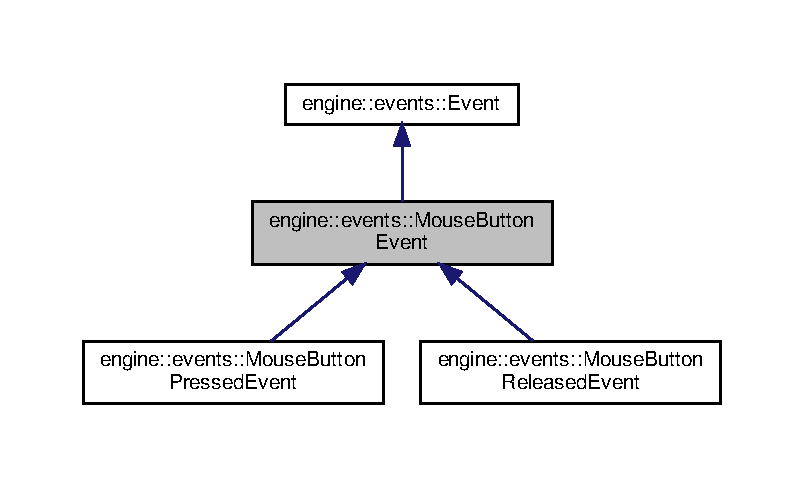
\includegraphics[width=350pt]{classengine_1_1events_1_1MouseButtonEvent__inherit__graph}
\end{center}
\end{figure}


Collaboration diagram for engine\+::events\+::Mouse\+Button\+Event\+:\nopagebreak
\begin{figure}[H]
\begin{center}
\leavevmode
\includegraphics[width=239pt]{classengine_1_1events_1_1MouseButtonEvent__coll__graph}
\end{center}
\end{figure}
\doxysubsection*{Public Member Functions}
\begin{DoxyCompactItemize}
\item 
\mbox{\Hypertarget{classengine_1_1events_1_1MouseButtonEvent_ad6e5db5a8f746d3e0da996246f4df035}\label{classengine_1_1events_1_1MouseButtonEvent_ad6e5db5a8f746d3e0da996246f4df035}} 
int {\bfseries Get\+Mouse\+Button} () const
\item 
\mbox{\Hypertarget{classengine_1_1events_1_1MouseButtonEvent_a7c6def7727370e4d850806c0b6fd5379}\label{classengine_1_1events_1_1MouseButtonEvent_a7c6def7727370e4d850806c0b6fd5379}} 
{\bfseries E\+V\+E\+N\+T\+\_\+\+C\+L\+A\+S\+S\+\_\+\+C\+A\+T\+E\+G\+O\+RY} (k\+Event\+Category\+Mouse$\vert$k\+Event\+Category\+Input) protected
\end{DoxyCompactItemize}
\doxysubsection*{Public Attributes}
\begin{DoxyCompactItemize}
\item 
\mbox{\Hypertarget{classengine_1_1events_1_1MouseButtonEvent_ac8f03e2926022023b87a713cb44e85b7}\label{classengine_1_1events_1_1MouseButtonEvent_ac8f03e2926022023b87a713cb44e85b7}} 
int {\bfseries button\+\_\+}
\end{DoxyCompactItemize}
\doxysubsection*{Additional Inherited Members}


\doxysubsection{Detailed Description}
The generic Mouse button event. 

The documentation for this class was generated from the following file\+:\begin{DoxyCompactItemize}
\item 
engine/src/core/events/\mbox{\hyperlink{MouseEvent_8h}{Mouse\+Event.\+h}}\end{DoxyCompactItemize}

\hypertarget{classengine_1_1events_1_1MouseButtonPressedEvent}{}\section{engine\+:\+:events\+:\+:Mouse\+Button\+Pressed\+Event Class Reference}
\label{classengine_1_1events_1_1MouseButtonPressedEvent}\index{engine\+::events\+::\+Mouse\+Button\+Pressed\+Event@{engine\+::events\+::\+Mouse\+Button\+Pressed\+Event}}


Generated whenever the user presses a mouse button within the application.  




{\ttfamily \#include $<$Mouse\+Event.\+h$>$}



Inheritance diagram for engine\+:\+:events\+:\+:Mouse\+Button\+Pressed\+Event\+:\nopagebreak
\begin{figure}[H]
\begin{center}
\leavevmode
\includegraphics[width=224pt]{classengine_1_1events_1_1MouseButtonPressedEvent__inherit__graph}
\end{center}
\end{figure}


Collaboration diagram for engine\+:\+:events\+:\+:Mouse\+Button\+Pressed\+Event\+:\nopagebreak
\begin{figure}[H]
\begin{center}
\leavevmode
\includegraphics[width=224pt]{classengine_1_1events_1_1MouseButtonPressedEvent__coll__graph}
\end{center}
\end{figure}
\subsection*{Public Member Functions}
\begin{DoxyCompactItemize}
\item 
\mbox{\Hypertarget{classengine_1_1events_1_1MouseButtonPressedEvent_a5c49d839717df26588e125e3defd28db}\label{classengine_1_1events_1_1MouseButtonPressedEvent_a5c49d839717df26588e125e3defd28db}} 
{\bfseries Mouse\+Button\+Pressed\+Event} (int button)
\item 
\mbox{\Hypertarget{classengine_1_1events_1_1MouseButtonPressedEvent_a51cb2a71b84c923d4205331686f7dc7d}\label{classengine_1_1events_1_1MouseButtonPressedEvent_a51cb2a71b84c923d4205331686f7dc7d}} 
std\+::string {\bfseries To\+String} () const override
\end{DoxyCompactItemize}
\subsection*{Additional Inherited Members}


\subsection{Detailed Description}
Generated whenever the user presses a mouse button within the application. 

The documentation for this class was generated from the following file\+:\begin{DoxyCompactItemize}
\item 
engine/src/core/events/\hyperlink{MouseEvent_8h}{Mouse\+Event.\+h}\end{DoxyCompactItemize}

\hypertarget{classengine_1_1events_1_1MouseButtonReleasedEvent}{}\doxysection{engine\+::events\+::Mouse\+Button\+Released\+Event Class Reference}
\label{classengine_1_1events_1_1MouseButtonReleasedEvent}\index{engine::events::MouseButtonReleasedEvent@{engine::events::MouseButtonReleasedEvent}}


Generated whenever the user releases a mouse button within an application.  




{\ttfamily \#include $<$Mouse\+Event.\+h$>$}



Inheritance diagram for engine\+::events\+::Mouse\+Button\+Released\+Event\+:\nopagebreak
\begin{figure}[H]
\begin{center}
\leavevmode
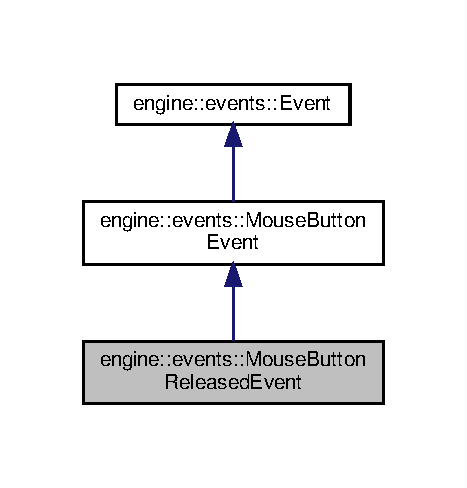
\includegraphics[width=239pt]{classengine_1_1events_1_1MouseButtonReleasedEvent__inherit__graph}
\end{center}
\end{figure}


Collaboration diagram for engine\+::events\+::Mouse\+Button\+Released\+Event\+:\nopagebreak
\begin{figure}[H]
\begin{center}
\leavevmode
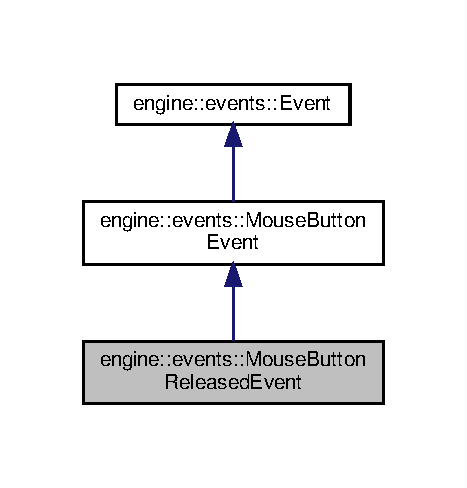
\includegraphics[width=239pt]{classengine_1_1events_1_1MouseButtonReleasedEvent__coll__graph}
\end{center}
\end{figure}
\doxysubsection*{Public Member Functions}
\begin{DoxyCompactItemize}
\item 
\mbox{\Hypertarget{classengine_1_1events_1_1MouseButtonReleasedEvent_a11f83d0912db1dc81c4bd8b69a5e33c3}\label{classengine_1_1events_1_1MouseButtonReleasedEvent_a11f83d0912db1dc81c4bd8b69a5e33c3}} 
{\bfseries Mouse\+Button\+Released\+Event} (int button)
\item 
\mbox{\Hypertarget{classengine_1_1events_1_1MouseButtonReleasedEvent_ae1cd60e0cad5a31fc6baaa15944fd212}\label{classengine_1_1events_1_1MouseButtonReleasedEvent_ae1cd60e0cad5a31fc6baaa15944fd212}} 
std\+::string {\bfseries To\+String} () const override
\end{DoxyCompactItemize}
\doxysubsection*{Additional Inherited Members}


\doxysubsection{Detailed Description}
Generated whenever the user releases a mouse button within an application. 

The documentation for this class was generated from the following file\+:\begin{DoxyCompactItemize}
\item 
engine/src/core/events/\mbox{\hyperlink{MouseEvent_8h}{Mouse\+Event.\+h}}\end{DoxyCompactItemize}

\hypertarget{classengine_1_1events_1_1MouseMovedEvent}{}\doxysection{engine\+::events\+::Mouse\+Moved\+Event Class Reference}
\label{classengine_1_1events_1_1MouseMovedEvent}\index{engine::events::MouseMovedEvent@{engine::events::MouseMovedEvent}}


Generated whenever the user moves their mouse within the application.  




{\ttfamily \#include $<$Mouse\+Event.\+h$>$}



Inheritance diagram for engine\+::events\+::Mouse\+Moved\+Event\+:\nopagebreak
\begin{figure}[H]
\begin{center}
\leavevmode
\includegraphics[width=240pt]{classengine_1_1events_1_1MouseMovedEvent__inherit__graph}
\end{center}
\end{figure}


Collaboration diagram for engine\+::events\+::Mouse\+Moved\+Event\+:\nopagebreak
\begin{figure}[H]
\begin{center}
\leavevmode
\includegraphics[width=240pt]{classengine_1_1events_1_1MouseMovedEvent__coll__graph}
\end{center}
\end{figure}
\doxysubsection*{Public Member Functions}
\begin{DoxyCompactItemize}
\item 
\mbox{\Hypertarget{classengine_1_1events_1_1MouseMovedEvent_a970a64e27a0d4dc882e07d18e31c9e88}\label{classengine_1_1events_1_1MouseMovedEvent_a970a64e27a0d4dc882e07d18e31c9e88}} 
{\bfseries Mouse\+Moved\+Event} (float x, float y)
\item 
\mbox{\Hypertarget{classengine_1_1events_1_1MouseMovedEvent_a6d8a932ee6d337f3d18fafb12805c4c4}\label{classengine_1_1events_1_1MouseMovedEvent_a6d8a932ee6d337f3d18fafb12805c4c4}} 
float {\bfseries GetX} () const
\item 
\mbox{\Hypertarget{classengine_1_1events_1_1MouseMovedEvent_a6f0d99a80de44d2bdd45d319bdfaa3f4}\label{classengine_1_1events_1_1MouseMovedEvent_a6f0d99a80de44d2bdd45d319bdfaa3f4}} 
float {\bfseries GetY} () const
\item 
\mbox{\Hypertarget{classengine_1_1events_1_1MouseMovedEvent_a9e8339925959fd0226b7c4cd1aa12fd3}\label{classengine_1_1events_1_1MouseMovedEvent_a9e8339925959fd0226b7c4cd1aa12fd3}} 
std\+::string {\bfseries To\+String} () const override
\end{DoxyCompactItemize}
\doxysubsection*{Additional Inherited Members}


\doxysubsection{Detailed Description}
Generated whenever the user moves their mouse within the application. 

The documentation for this class was generated from the following file\+:\begin{DoxyCompactItemize}
\item 
engine/src/core/events/\mbox{\hyperlink{MouseEvent_8h}{Mouse\+Event.\+h}}\end{DoxyCompactItemize}

\hypertarget{classengine_1_1events_1_1MouseScrolledEvent}{}\section{engine\+:\+:events\+:\+:Mouse\+Scrolled\+Event Class Reference}
\label{classengine_1_1events_1_1MouseScrolledEvent}\index{engine\+::events\+::\+Mouse\+Scrolled\+Event@{engine\+::events\+::\+Mouse\+Scrolled\+Event}}


Inheritance diagram for engine\+:\+:events\+:\+:Mouse\+Scrolled\+Event\+:
\nopagebreak
\begin{figure}[H]
\begin{center}
\leavevmode
\includegraphics[width=231pt]{classengine_1_1events_1_1MouseScrolledEvent__inherit__graph}
\end{center}
\end{figure}


Collaboration diagram for engine\+:\+:events\+:\+:Mouse\+Scrolled\+Event\+:
\nopagebreak
\begin{figure}[H]
\begin{center}
\leavevmode
\includegraphics[width=231pt]{classengine_1_1events_1_1MouseScrolledEvent__coll__graph}
\end{center}
\end{figure}
\subsection*{Public Member Functions}
\begin{DoxyCompactItemize}
\item
\mbox{\Hypertarget{classengine_1_1events_1_1MouseScrolledEvent_ad118d6e0e1b9e17e8853139af451f972}\label{classengine_1_1events_1_1MouseScrolledEvent_ad118d6e0e1b9e17e8853139af451f972}}
{\bfseries Mouse\+Scrolled\+Event} (float x\+\_\+offset, float y\+\_\+offset)
\item
\mbox{\Hypertarget{classengine_1_1events_1_1MouseScrolledEvent_a6811c762e35b9aa99efb92629f624d37}\label{classengine_1_1events_1_1MouseScrolledEvent_a6811c762e35b9aa99efb92629f624d37}}
float {\bfseries Get\+X\+Offset} () const
\item
\mbox{\Hypertarget{classengine_1_1events_1_1MouseScrolledEvent_ac8497ef915ec94c1bca1646550ac0f45}\label{classengine_1_1events_1_1MouseScrolledEvent_ac8497ef915ec94c1bca1646550ac0f45}}
float {\bfseries Get\+Y\+Offset} () const
\item
\mbox{\Hypertarget{classengine_1_1events_1_1MouseScrolledEvent_aac2386bd24310ea41ce995134614aba9}\label{classengine_1_1events_1_1MouseScrolledEvent_aac2386bd24310ea41ce995134614aba9}}
std\+::string {\bfseries To\+String} () const override
\end{DoxyCompactItemize}
\subsection*{Additional Inherited Members}


The documentation for this class was generated from the following file\+:\begin{DoxyCompactItemize}
\item
engine/src/core/events/Mouse\+Event.\+h\end{DoxyCompactItemize}

\hypertarget{classengine_1_1platform_1_1opengl_1_1OpenGLContext}{}\section{engine\+:\+:platform\+:\+:opengl\+:\+:Open\+G\+L\+Context Class Reference}
\label{classengine_1_1platform_1_1opengl_1_1OpenGLContext}\index{engine\+::platform\+::opengl\+::\+Open\+G\+L\+Context@{engine\+::platform\+::opengl\+::\+Open\+G\+L\+Context}}


Inheritance diagram for engine\+:\+:platform\+:\+:opengl\+:\+:Open\+G\+L\+Context\+:
\nopagebreak
\begin{figure}[H]
\begin{center}
\leavevmode
\includegraphics[width=211pt]{classengine_1_1platform_1_1opengl_1_1OpenGLContext__inherit__graph}
\end{center}
\end{figure}


Collaboration diagram for engine\+:\+:platform\+:\+:opengl\+:\+:Open\+G\+L\+Context\+:
\nopagebreak
\begin{figure}[H]
\begin{center}
\leavevmode
\includegraphics[width=211pt]{classengine_1_1platform_1_1opengl_1_1OpenGLContext__coll__graph}
\end{center}
\end{figure}
\subsection*{Public Member Functions}
\begin{DoxyCompactItemize}
\item 
\mbox{\Hypertarget{classengine_1_1platform_1_1opengl_1_1OpenGLContext_a37878633b98b04e889751132ca7a5845}\label{classengine_1_1platform_1_1opengl_1_1OpenGLContext_a37878633b98b04e889751132ca7a5845}} 
{\bfseries Open\+G\+L\+Context} (G\+L\+F\+Wwindow $\ast$window\+\_\+handle)
\item 
\mbox{\Hypertarget{classengine_1_1platform_1_1opengl_1_1OpenGLContext_a9243aaae6fab53ef1985dbd81785aca0}\label{classengine_1_1platform_1_1opengl_1_1OpenGLContext_a9243aaae6fab53ef1985dbd81785aca0}} 
void {\bfseries Init} () override
\item 
\mbox{\Hypertarget{classengine_1_1platform_1_1opengl_1_1OpenGLContext_a4d063b45f3915f10a2f82d1a5f301483}\label{classengine_1_1platform_1_1opengl_1_1OpenGLContext_a4d063b45f3915f10a2f82d1a5f301483}} 
void {\bfseries Swap\+Buffers} () override
\end{DoxyCompactItemize}


The documentation for this class was generated from the following files\+:\begin{DoxyCompactItemize}
\item 
engine/src/platform/opengl/Open\+G\+L\+Context.\+h\item 
engine/src/platform/opengl/Open\+G\+L\+Context.\+cpp\end{DoxyCompactItemize}

\hypertarget{classengine_1_1platform_1_1opengl_1_1OpenGLIndexBuffer}{}\doxysection{engine\+::platform\+::opengl\+::Open\+G\+L\+Index\+Buffer Class Reference}
\label{classengine_1_1platform_1_1opengl_1_1OpenGLIndexBuffer}\index{engine::platform::opengl::OpenGLIndexBuffer@{engine::platform::opengl::OpenGLIndexBuffer}}


Inheritance diagram for engine\+::platform\+::opengl\+::Open\+G\+L\+Index\+Buffer\+:\nopagebreak
\begin{figure}[H]
\begin{center}
\leavevmode
\includegraphics[width=240pt]{classengine_1_1platform_1_1opengl_1_1OpenGLIndexBuffer__inherit__graph}
\end{center}
\end{figure}


Collaboration diagram for engine\+::platform\+::opengl\+::Open\+G\+L\+Index\+Buffer\+:\nopagebreak
\begin{figure}[H]
\begin{center}
\leavevmode
\includegraphics[width=240pt]{classengine_1_1platform_1_1opengl_1_1OpenGLIndexBuffer__coll__graph}
\end{center}
\end{figure}
\doxysubsection*{Public Member Functions}
\begin{DoxyCompactItemize}
\item 
\mbox{\hyperlink{classengine_1_1platform_1_1opengl_1_1OpenGLIndexBuffer_a88830d5185f3fd37d8274029f8d78746}{Open\+G\+L\+Index\+Buffer}} (uint32\+\_\+t $\ast$indices, uint32\+\_\+t count)
\item 
\mbox{\Hypertarget{classengine_1_1platform_1_1opengl_1_1OpenGLIndexBuffer_ad9279e716132e186a38fe82814f29b0f}\label{classengine_1_1platform_1_1opengl_1_1OpenGLIndexBuffer_ad9279e716132e186a38fe82814f29b0f}} 
void \mbox{\hyperlink{classengine_1_1platform_1_1opengl_1_1OpenGLIndexBuffer_ad9279e716132e186a38fe82814f29b0f}{Bind}} () const override
\begin{DoxyCompactList}\small\item\em Bind the current Index\+Buffer to the current rendering context. \end{DoxyCompactList}\item 
void \mbox{\hyperlink{classengine_1_1platform_1_1opengl_1_1OpenGLIndexBuffer_a9fc400e4c464a2dbf7df76eba359639e}{Unbind}} () const override
\begin{DoxyCompactList}\small\item\em Unbind the current Index\+Buffer from the current rendering context. \end{DoxyCompactList}\item 
\mbox{\Hypertarget{classengine_1_1platform_1_1opengl_1_1OpenGLIndexBuffer_a2353743de19ca153e5e1123ef0132952}\label{classengine_1_1platform_1_1opengl_1_1OpenGLIndexBuffer_a2353743de19ca153e5e1123ef0132952}} 
uint32\+\_\+t \mbox{\hyperlink{classengine_1_1platform_1_1opengl_1_1OpenGLIndexBuffer_a2353743de19ca153e5e1123ef0132952}{Get\+Count}} () const override
\begin{DoxyCompactList}\small\item\em Get the count of indices within the current Index\+Buffer. \end{DoxyCompactList}\end{DoxyCompactItemize}
\doxysubsection*{Additional Inherited Members}


\doxysubsection{Constructor \& Destructor Documentation}
\mbox{\Hypertarget{classengine_1_1platform_1_1opengl_1_1OpenGLIndexBuffer_a88830d5185f3fd37d8274029f8d78746}\label{classengine_1_1platform_1_1opengl_1_1OpenGLIndexBuffer_a88830d5185f3fd37d8274029f8d78746}} 
\index{engine::platform::opengl::OpenGLIndexBuffer@{engine::platform::opengl::OpenGLIndexBuffer}!OpenGLIndexBuffer@{OpenGLIndexBuffer}}
\index{OpenGLIndexBuffer@{OpenGLIndexBuffer}!engine::platform::opengl::OpenGLIndexBuffer@{engine::platform::opengl::OpenGLIndexBuffer}}
\doxysubsubsection{\texorpdfstring{OpenGLIndexBuffer()}{OpenGLIndexBuffer()}}
{\footnotesize\ttfamily engine\+::platform\+::opengl\+::\+Open\+G\+L\+Index\+Buffer\+::\+Open\+G\+L\+Index\+Buffer (\begin{DoxyParamCaption}\item[{uint32\+\_\+t $\ast$}]{indices,  }\item[{uint32\+\_\+t}]{count }\end{DoxyParamCaption})}

Constructs an Index buffer given an array of indices and total count. The instantiation of the index buffer will cause the engine to to assert an error if the count is $>$ 0. 

\doxysubsection{Member Function Documentation}
\mbox{\Hypertarget{classengine_1_1platform_1_1opengl_1_1OpenGLIndexBuffer_a9fc400e4c464a2dbf7df76eba359639e}\label{classengine_1_1platform_1_1opengl_1_1OpenGLIndexBuffer_a9fc400e4c464a2dbf7df76eba359639e}} 
\index{engine::platform::opengl::OpenGLIndexBuffer@{engine::platform::opengl::OpenGLIndexBuffer}!Unbind@{Unbind}}
\index{Unbind@{Unbind}!engine::platform::opengl::OpenGLIndexBuffer@{engine::platform::opengl::OpenGLIndexBuffer}}
\doxysubsubsection{\texorpdfstring{Unbind()}{Unbind()}}
{\footnotesize\ttfamily void engine\+::platform\+::opengl\+::\+Open\+G\+L\+Index\+Buffer\+::\+Unbind (\begin{DoxyParamCaption}{ }\end{DoxyParamCaption}) const\hspace{0.3cm}{\ttfamily [override]}, {\ttfamily [virtual]}}



Unbind the current Index\+Buffer from the current rendering context. 

Any vertex buffer that relies on this buffer will not be able to access the contents of it once unbound from the graphics context. 

Implements \mbox{\hyperlink{classengine_1_1renderer_1_1IndexBuffer_a8fd1ab43d3963533370c4d8e2e2282f4}{engine\+::renderer\+::\+Index\+Buffer}}.



The documentation for this class was generated from the following files\+:\begin{DoxyCompactItemize}
\item 
engine/src/platform/opengl/Open\+G\+L\+Buffer.\+h\item 
engine/src/platform/opengl/Open\+G\+L\+Buffer.\+cpp\end{DoxyCompactItemize}

\hypertarget{classengine_1_1platform_1_1opengl_1_1OpenGLVertexBuffer}{}\section{engine\+:\+:platform\+:\+:opengl\+:\+:Open\+G\+L\+Vertex\+Buffer Class Reference}
\label{classengine_1_1platform_1_1opengl_1_1OpenGLVertexBuffer}\index{engine\+::platform\+::opengl\+::\+Open\+G\+L\+Vertex\+Buffer@{engine\+::platform\+::opengl\+::\+Open\+G\+L\+Vertex\+Buffer}}


{\ttfamily \#include $<$Open\+G\+L\+Buffer.\+h$>$}



Inheritance diagram for engine\+:\+:platform\+:\+:opengl\+:\+:Open\+G\+L\+Vertex\+Buffer\+:\nopagebreak
\begin{figure}[H]
\begin{center}
\leavevmode
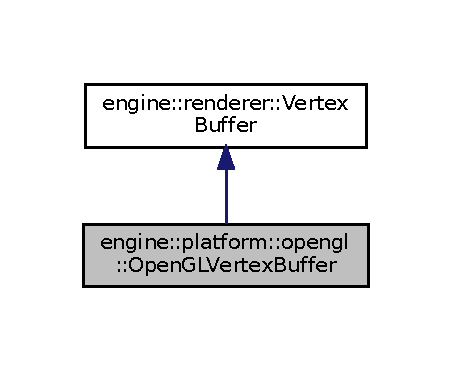
\includegraphics[width=201pt]{classengine_1_1platform_1_1opengl_1_1OpenGLVertexBuffer__inherit__graph}
\end{center}
\end{figure}


Collaboration diagram for engine\+:\+:platform\+:\+:opengl\+:\+:Open\+G\+L\+Vertex\+Buffer\+:\nopagebreak
\begin{figure}[H]
\begin{center}
\leavevmode
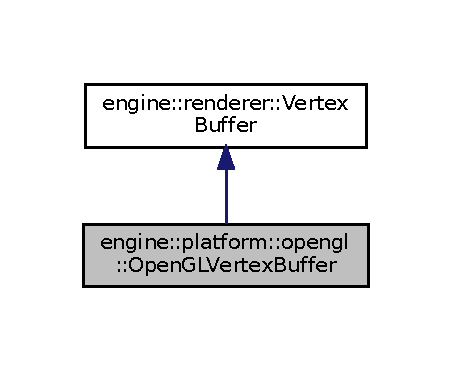
\includegraphics[width=201pt]{classengine_1_1platform_1_1opengl_1_1OpenGLVertexBuffer__coll__graph}
\end{center}
\end{figure}
\subsection*{Public Member Functions}
\begin{DoxyCompactItemize}
\item 
\mbox{\Hypertarget{classengine_1_1platform_1_1opengl_1_1OpenGLVertexBuffer_a481164805afb44795f3e545e07c3b3bc}\label{classengine_1_1platform_1_1opengl_1_1OpenGLVertexBuffer_a481164805afb44795f3e545e07c3b3bc}} 
{\bfseries Open\+G\+L\+Vertex\+Buffer} (float $\ast$vertices, uint32\+\_\+t size)
\item 
void \hyperlink{classengine_1_1platform_1_1opengl_1_1OpenGLVertexBuffer_ac50918719a747f81d7fe94dfcc8dec13}{Bind} () const override
\item 
void \hyperlink{classengine_1_1platform_1_1opengl_1_1OpenGLVertexBuffer_a9069ca746c0de9dd9418ba9c5ee7b67b}{Unbind} () const override
\item 
const \hyperlink{classengine_1_1renderer_1_1BufferLayout}{renderer\+::\+Buffer\+Layout} \& \hyperlink{classengine_1_1platform_1_1opengl_1_1OpenGLVertexBuffer_a0d4f81503171f6bbe41ece0fada23390}{Get\+Layout} () const override
\item 
void \hyperlink{classengine_1_1platform_1_1opengl_1_1OpenGLVertexBuffer_a957a9dc55dc35ce4302654e1a394e5f8}{Set\+Layout} (const \hyperlink{classengine_1_1renderer_1_1BufferLayout}{renderer\+::\+Buffer\+Layout} \&layout) override
\end{DoxyCompactItemize}
\subsection*{Additional Inherited Members}


\subsection{Detailed Description}
The Open\+GL Vertex\+Buffer implementation based off the generic Vertex\+Buffer base class provided by the engines renderer. 

\subsection{Member Function Documentation}
\mbox{\Hypertarget{classengine_1_1platform_1_1opengl_1_1OpenGLVertexBuffer_ac50918719a747f81d7fe94dfcc8dec13}\label{classengine_1_1platform_1_1opengl_1_1OpenGLVertexBuffer_ac50918719a747f81d7fe94dfcc8dec13}} 
\index{engine\+::platform\+::opengl\+::\+Open\+G\+L\+Vertex\+Buffer@{engine\+::platform\+::opengl\+::\+Open\+G\+L\+Vertex\+Buffer}!Bind@{Bind}}
\index{Bind@{Bind}!engine\+::platform\+::opengl\+::\+Open\+G\+L\+Vertex\+Buffer@{engine\+::platform\+::opengl\+::\+Open\+G\+L\+Vertex\+Buffer}}
\subsubsection{\texorpdfstring{Bind()}{Bind()}}
{\footnotesize\ttfamily void engine\+::platform\+::opengl\+::\+Open\+G\+L\+Vertex\+Buffer\+::\+Bind (\begin{DoxyParamCaption}{ }\end{DoxyParamCaption}) const\hspace{0.3cm}{\ttfamily [override]}, {\ttfamily [virtual]}}

Create and bind the vertex buffer on the G\+PU. Will set the renderer\+\_\+\+I\+D\+\_\+. 

Implements \hyperlink{classengine_1_1renderer_1_1VertexBuffer_a62c7bd816aa10b69d1e903918ecc4414}{engine\+::renderer\+::\+Vertex\+Buffer}.

\mbox{\Hypertarget{classengine_1_1platform_1_1opengl_1_1OpenGLVertexBuffer_a0d4f81503171f6bbe41ece0fada23390}\label{classengine_1_1platform_1_1opengl_1_1OpenGLVertexBuffer_a0d4f81503171f6bbe41ece0fada23390}} 
\index{engine\+::platform\+::opengl\+::\+Open\+G\+L\+Vertex\+Buffer@{engine\+::platform\+::opengl\+::\+Open\+G\+L\+Vertex\+Buffer}!Get\+Layout@{Get\+Layout}}
\index{Get\+Layout@{Get\+Layout}!engine\+::platform\+::opengl\+::\+Open\+G\+L\+Vertex\+Buffer@{engine\+::platform\+::opengl\+::\+Open\+G\+L\+Vertex\+Buffer}}
\subsubsection{\texorpdfstring{Get\+Layout()}{GetLayout()}}
{\footnotesize\ttfamily const \hyperlink{classengine_1_1renderer_1_1BufferLayout}{renderer\+::\+Buffer\+Layout}\& engine\+::platform\+::opengl\+::\+Open\+G\+L\+Vertex\+Buffer\+::\+Get\+Layout (\begin{DoxyParamCaption}{ }\end{DoxyParamCaption}) const\hspace{0.3cm}{\ttfamily [inline]}, {\ttfamily [override]}, {\ttfamily [virtual]}}

Get the Buffer\+Layout associated with the current Vertex\+Buffer. 

Implements \hyperlink{classengine_1_1renderer_1_1VertexBuffer_a3186b40aa8c8c471fe80c29645859aa5}{engine\+::renderer\+::\+Vertex\+Buffer}.

\mbox{\Hypertarget{classengine_1_1platform_1_1opengl_1_1OpenGLVertexBuffer_a957a9dc55dc35ce4302654e1a394e5f8}\label{classengine_1_1platform_1_1opengl_1_1OpenGLVertexBuffer_a957a9dc55dc35ce4302654e1a394e5f8}} 
\index{engine\+::platform\+::opengl\+::\+Open\+G\+L\+Vertex\+Buffer@{engine\+::platform\+::opengl\+::\+Open\+G\+L\+Vertex\+Buffer}!Set\+Layout@{Set\+Layout}}
\index{Set\+Layout@{Set\+Layout}!engine\+::platform\+::opengl\+::\+Open\+G\+L\+Vertex\+Buffer@{engine\+::platform\+::opengl\+::\+Open\+G\+L\+Vertex\+Buffer}}
\subsubsection{\texorpdfstring{Set\+Layout()}{SetLayout()}}
{\footnotesize\ttfamily void engine\+::platform\+::opengl\+::\+Open\+G\+L\+Vertex\+Buffer\+::\+Set\+Layout (\begin{DoxyParamCaption}\item[{const \hyperlink{classengine_1_1renderer_1_1BufferLayout}{renderer\+::\+Buffer\+Layout} \&}]{layout }\end{DoxyParamCaption})\hspace{0.3cm}{\ttfamily [inline]}, {\ttfamily [override]}, {\ttfamily [virtual]}}

Set the Buffer\+Layout associated with the current Vertex\+Buffer. 

Implements \hyperlink{classengine_1_1renderer_1_1VertexBuffer_afad191b22fec9bc2519e43d543e5c75e}{engine\+::renderer\+::\+Vertex\+Buffer}.

\mbox{\Hypertarget{classengine_1_1platform_1_1opengl_1_1OpenGLVertexBuffer_a9069ca746c0de9dd9418ba9c5ee7b67b}\label{classengine_1_1platform_1_1opengl_1_1OpenGLVertexBuffer_a9069ca746c0de9dd9418ba9c5ee7b67b}} 
\index{engine\+::platform\+::opengl\+::\+Open\+G\+L\+Vertex\+Buffer@{engine\+::platform\+::opengl\+::\+Open\+G\+L\+Vertex\+Buffer}!Unbind@{Unbind}}
\index{Unbind@{Unbind}!engine\+::platform\+::opengl\+::\+Open\+G\+L\+Vertex\+Buffer@{engine\+::platform\+::opengl\+::\+Open\+G\+L\+Vertex\+Buffer}}
\subsubsection{\texorpdfstring{Unbind()}{Unbind()}}
{\footnotesize\ttfamily void engine\+::platform\+::opengl\+::\+Open\+G\+L\+Vertex\+Buffer\+::\+Unbind (\begin{DoxyParamCaption}{ }\end{DoxyParamCaption}) const\hspace{0.3cm}{\ttfamily [override]}, {\ttfamily [virtual]}}

Unbind and delete the vertex buffer on G\+PU using the renderer\+\_\+\+I\+D\+\_\+ associated with it. 

Implements \hyperlink{classengine_1_1renderer_1_1VertexBuffer_a06b240b93506dfd383b3a3f8947eb26f}{engine\+::renderer\+::\+Vertex\+Buffer}.



The documentation for this class was generated from the following files\+:\begin{DoxyCompactItemize}
\item 
engine/src/platform/opengl/Open\+G\+L\+Buffer.\+h\item 
engine/src/platform/opengl/Open\+G\+L\+Buffer.\+cpp\end{DoxyCompactItemize}

\hypertarget{classengine_1_1renderer_1_1Renderer}{}\doxysection{engine\+::renderer\+::Renderer Class Reference}
\label{classengine_1_1renderer_1_1Renderer}\index{engine::renderer::Renderer@{engine::renderer::Renderer}}


A lightweight rendering A\+PI implementation. Allows generalized calls to be written for users.  




{\ttfamily \#include $<$Renderer.\+h$>$}

\doxysubsection*{Static Public Member Functions}
\begin{DoxyCompactItemize}
\item 
\mbox{\Hypertarget{classengine_1_1renderer_1_1Renderer_a07fcd1f8a780b8ef8fcb01dc97dc0db9}\label{classengine_1_1renderer_1_1Renderer_a07fcd1f8a780b8ef8fcb01dc97dc0db9}} 
static void \mbox{\hyperlink{classengine_1_1renderer_1_1Renderer_a07fcd1f8a780b8ef8fcb01dc97dc0db9}{Begin\+Scene}} (const \mbox{\hyperlink{classengine_1_1renderer_1_1OrthographicCamera}{Orthographic\+Camera}} \&camera)
\begin{DoxyCompactList}\small\item\em Begin rendering a scene. \end{DoxyCompactList}\item 
\mbox{\Hypertarget{classengine_1_1renderer_1_1Renderer_a02a319a6fac8e3dc13b492976c4ad5d3}\label{classengine_1_1renderer_1_1Renderer_a02a319a6fac8e3dc13b492976c4ad5d3}} 
static void \mbox{\hyperlink{classengine_1_1renderer_1_1Renderer_a02a319a6fac8e3dc13b492976c4ad5d3}{End\+Scene}} ()
\begin{DoxyCompactList}\small\item\em Stop rendering a scene. \end{DoxyCompactList}\item 
static void \mbox{\hyperlink{classengine_1_1renderer_1_1Renderer_a9c843a2327a60bbd2226c717a3e6dd1a}{Submit}} (const std\+::shared\+\_\+ptr$<$ \mbox{\hyperlink{classengine_1_1renderer_1_1VertexArray}{Vertex\+Array}} $>$ \&vertex\+\_\+array, const std\+::shared\+\_\+ptr$<$ \mbox{\hyperlink{classengine_1_1renderer_1_1Shader}{Shader}} $>$ \&shader, const glm\+::mat4 \&transform=glm\+::mat4(1.\+0f))
\begin{DoxyCompactList}\small\item\em Submit a scene data to the engine. \end{DoxyCompactList}\item 
\mbox{\Hypertarget{classengine_1_1renderer_1_1Renderer_a61d12573cda993102d8e335f17380c8a}\label{classengine_1_1renderer_1_1Renderer_a61d12573cda993102d8e335f17380c8a}} 
static \mbox{\hyperlink{classengine_1_1renderer_1_1RendererAPI_a624c2793dc8b315466c36332bbc82ef0}{Renderer\+A\+P\+I\+::\+A\+PI}} {\bfseries Get\+A\+PI} ()
\end{DoxyCompactItemize}


\doxysubsection{Detailed Description}
A lightweight rendering A\+PI implementation. Allows generalized calls to be written for users. 

A lightweight and not fully finished rendering A\+PI that lets you set the a specific graphics context to use for rendering. This must be set externally in any rendering application. 

\doxysubsection{Member Function Documentation}
\mbox{\Hypertarget{classengine_1_1renderer_1_1Renderer_a9c843a2327a60bbd2226c717a3e6dd1a}\label{classengine_1_1renderer_1_1Renderer_a9c843a2327a60bbd2226c717a3e6dd1a}} 
\index{engine::renderer::Renderer@{engine::renderer::Renderer}!Submit@{Submit}}
\index{Submit@{Submit}!engine::renderer::Renderer@{engine::renderer::Renderer}}
\doxysubsubsection{\texorpdfstring{Submit()}{Submit()}}
{\footnotesize\ttfamily engine\+::renderer\+::\+Renderer\+::\+Submit (\begin{DoxyParamCaption}\item[{const std\+::shared\+\_\+ptr$<$ \mbox{\hyperlink{classengine_1_1renderer_1_1VertexArray}{Vertex\+Array}} $>$ \&}]{vertex\+\_\+array,  }\item[{const std\+::shared\+\_\+ptr$<$ \mbox{\hyperlink{classengine_1_1renderer_1_1Shader}{Shader}} $>$ \&}]{shader,  }\item[{const glm\+::mat4 \&}]{transform = {\ttfamily glm\+:\+:mat4(1.0f)} }\end{DoxyParamCaption})\hspace{0.3cm}{\ttfamily [static]}}



Submit a scene data to the engine. 

Binds both the shader and vertex array before issuing a draw call. 

The documentation for this class was generated from the following files\+:\begin{DoxyCompactItemize}
\item 
engine/src/core/renderer/\mbox{\hyperlink{Renderer_8h}{Renderer.\+h}}\item 
engine/src/core/renderer/Renderer.\+cpp\end{DoxyCompactItemize}

\hypertarget{classengine_1_1renderer_1_1Shader}{}\doxysection{engine\+::renderer\+::Shader Class Reference}
\label{classengine_1_1renderer_1_1Shader}\index{engine::renderer::Shader@{engine::renderer::Shader}}


The abstract \mbox{\hyperlink{classengine_1_1renderer_1_1Shader}{Shader}} A\+PI.  




{\ttfamily \#include $<$Shader.\+h$>$}



Inheritance diagram for engine\+::renderer\+::Shader\+:\nopagebreak
\begin{figure}[H]
\begin{center}
\leavevmode
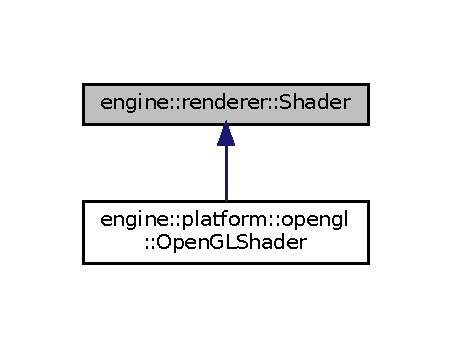
\includegraphics[width=217pt]{classengine_1_1renderer_1_1Shader__inherit__graph}
\end{center}
\end{figure}
\doxysubsection*{Public Member Functions}
\begin{DoxyCompactItemize}
\item 
\mbox{\Hypertarget{classengine_1_1renderer_1_1Shader_a3ed38f0ec020bc967a2ef6561e2f6d54}\label{classengine_1_1renderer_1_1Shader_a3ed38f0ec020bc967a2ef6561e2f6d54}} 
virtual void {\bfseries Bind} () const =0
\item 
\mbox{\Hypertarget{classengine_1_1renderer_1_1Shader_aa7daf0c5c60b4e0abe7ea105626bd66e}\label{classengine_1_1renderer_1_1Shader_aa7daf0c5c60b4e0abe7ea105626bd66e}} 
virtual void {\bfseries Unbind} () const =0
\end{DoxyCompactItemize}
\doxysubsection*{Static Public Member Functions}
\begin{DoxyCompactItemize}
\item 
\mbox{\Hypertarget{classengine_1_1renderer_1_1Shader_a575edd360f27be0eaa6434444f0072c5}\label{classengine_1_1renderer_1_1Shader_a575edd360f27be0eaa6434444f0072c5}} 
static \mbox{\hyperlink{classengine_1_1renderer_1_1Shader}{Shader}} $\ast$ {\bfseries Create} (const std\+::string \&vertex\+\_\+source, const std\+::string \&fragment\+\_\+source)
\end{DoxyCompactItemize}


\doxysubsection{Detailed Description}
The abstract \mbox{\hyperlink{classengine_1_1renderer_1_1Shader}{Shader}} A\+PI. 

The documentation for this class was generated from the following files\+:\begin{DoxyCompactItemize}
\item 
engine/src/core/renderer/\mbox{\hyperlink{Shader_8h}{Shader.\+h}}\item 
engine/src/core/renderer/Shader.\+cpp\end{DoxyCompactItemize}

\hypertarget{classengine_1_1renderer_1_1VertexBuffer}{}\section{engine\+:\+:renderer\+:\+:Vertex\+Buffer Class Reference}
\label{classengine_1_1renderer_1_1VertexBuffer}\index{engine\+::renderer\+::\+Vertex\+Buffer@{engine\+::renderer\+::\+Vertex\+Buffer}}


{\ttfamily \#include $<$Buffer.\+h$>$}



Inheritance diagram for engine\+:\+:renderer\+:\+:Vertex\+Buffer\+:\nopagebreak
\begin{figure}[H]
\begin{center}
\leavevmode
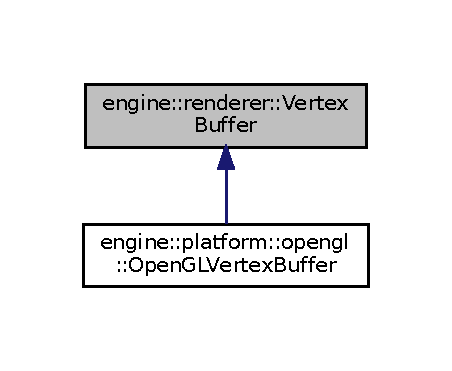
\includegraphics[width=201pt]{classengine_1_1renderer_1_1VertexBuffer__inherit__graph}
\end{center}
\end{figure}
\subsection*{Public Member Functions}
\begin{DoxyCompactItemize}
\item 
\mbox{\Hypertarget{classengine_1_1renderer_1_1VertexBuffer_acccb2af8de4a3a557f308757010a1fe7}\label{classengine_1_1renderer_1_1VertexBuffer_acccb2af8de4a3a557f308757010a1fe7}} 
virtual void {\bfseries Bind} () const =0
\item 
\mbox{\Hypertarget{classengine_1_1renderer_1_1VertexBuffer_ab2bc17d0e37c25c369367ea6b1137283}\label{classengine_1_1renderer_1_1VertexBuffer_ab2bc17d0e37c25c369367ea6b1137283}} 
virtual void {\bfseries Unbind} () const =0
\item 
\mbox{\Hypertarget{classengine_1_1renderer_1_1VertexBuffer_ab769bac40b3e30891fa4d5ee35ae6f2b}\label{classengine_1_1renderer_1_1VertexBuffer_ab769bac40b3e30891fa4d5ee35ae6f2b}} 
virtual const \hyperlink{classengine_1_1renderer_1_1BufferLayout}{Buffer\+Layout} \& {\bfseries Get\+Layout} () const =0
\item 
\mbox{\Hypertarget{classengine_1_1renderer_1_1VertexBuffer_a2885e3856bfb698178b6cd00a4dc7aab}\label{classengine_1_1renderer_1_1VertexBuffer_a2885e3856bfb698178b6cd00a4dc7aab}} 
virtual void {\bfseries Set\+Layout} (const \hyperlink{classengine_1_1renderer_1_1BufferLayout}{Buffer\+Layout} \&)=0
\end{DoxyCompactItemize}
\subsection*{Static Public Member Functions}
\begin{DoxyCompactItemize}
\item 
\mbox{\Hypertarget{classengine_1_1renderer_1_1VertexBuffer_ad7590ff8837ebcf2ed645f4a379e04d8}\label{classengine_1_1renderer_1_1VertexBuffer_ad7590ff8837ebcf2ed645f4a379e04d8}} 
static \hyperlink{classengine_1_1renderer_1_1VertexBuffer}{Vertex\+Buffer} $\ast$ {\bfseries Create} (float $\ast$vertices, uint32\+\_\+t size)
\end{DoxyCompactItemize}


\subsection{Detailed Description}
Generic \hyperlink{classengine_1_1renderer_1_1VertexBuffer}{Vertex\+Buffer} implementation to represent generalized Vertex buffers to be implemented for platform specific graphics libraries. 

The documentation for this class was generated from the following files\+:\begin{DoxyCompactItemize}
\item 
engine/src/core/renderer/Buffer.\+h\item 
engine/src/core/renderer/Buffer.\+cpp\end{DoxyCompactItemize}

\hypertarget{classengine_1_1Window}{}\section{engine\+:\+:Window Class Reference}
\label{classengine_1_1Window}\index{engine\+::\+Window@{engine\+::\+Window}}
\subsection*{Public Types}
\begin{DoxyCompactItemize}
\item 
\mbox{\Hypertarget{classengine_1_1Window_accae77cf11b87e90027b03c4fb9afe80}\label{classengine_1_1Window_accae77cf11b87e90027b03c4fb9afe80}} 
typedef std\+::function$<$ void(\hyperlink{classengine_1_1events_1_1Event}{events\+::\+Event} $\ast$)$>$ {\bfseries Event\+Callback\+Function}
\end{DoxyCompactItemize}
\subsection*{Public Member Functions}
\begin{DoxyCompactItemize}
\item 
\mbox{\Hypertarget{classengine_1_1Window_acbe42756a4062951c06a3d52970ffc70}\label{classengine_1_1Window_acbe42756a4062951c06a3d52970ffc70}} 
virtual void {\bfseries On\+Update} ()=0
\item 
\mbox{\Hypertarget{classengine_1_1Window_ab98eea2d4d31b19af72c452d932f51e7}\label{classengine_1_1Window_ab98eea2d4d31b19af72c452d932f51e7}} 
virtual unsigned int {\bfseries Get\+Width} () const =0
\item 
\mbox{\Hypertarget{classengine_1_1Window_aaa222cfbb6047cf6bf0337a94f5bdab0}\label{classengine_1_1Window_aaa222cfbb6047cf6bf0337a94f5bdab0}} 
virtual unsigned int {\bfseries Get\+Height} () const =0
\item 
\mbox{\Hypertarget{classengine_1_1Window_a7c66a5afd9dbfcc99782847c71826eac}\label{classengine_1_1Window_a7c66a5afd9dbfcc99782847c71826eac}} 
virtual void {\bfseries Set\+Event\+Callback} (const Event\+Callback\+Function \&callback)=0
\item 
\mbox{\Hypertarget{classengine_1_1Window_a671eb924c7114d991ed24f0e24325517}\label{classengine_1_1Window_a671eb924c7114d991ed24f0e24325517}} 
virtual void {\bfseries Set\+Vertical\+Sync} (bool enabled)=0
\item 
\mbox{\Hypertarget{classengine_1_1Window_a62914a8d91d0c1891a3168a61e5a59ba}\label{classengine_1_1Window_a62914a8d91d0c1891a3168a61e5a59ba}} 
virtual bool {\bfseries Has\+Vertical\+Sync} () const =0
\item 
\mbox{\Hypertarget{classengine_1_1Window_aa13831c03659b38bd405371b409c13d0}\label{classengine_1_1Window_aa13831c03659b38bd405371b409c13d0}} 
virtual void $\ast$ {\bfseries Get\+Native\+Window} () const =0
\end{DoxyCompactItemize}
\subsection*{Static Public Member Functions}
\begin{DoxyCompactItemize}
\item 
\mbox{\Hypertarget{classengine_1_1Window_a325de6424cfdd7fb58c05679e595008a}\label{classengine_1_1Window_a325de6424cfdd7fb58c05679e595008a}} 
static \hyperlink{classengine_1_1Window}{Window} $\ast$ {\bfseries Create} (const \hyperlink{structengine_1_1WindowProperties}{Window\+Properties} \&properties=\hyperlink{structengine_1_1WindowProperties}{Window\+Properties}())
\end{DoxyCompactItemize}


The documentation for this class was generated from the following file\+:\begin{DoxyCompactItemize}
\item 
engine/src/core/Window.\+h\end{DoxyCompactItemize}

\hypertarget{classengine_1_1events_1_1WindowCloseEvent}{}\section{engine\+:\+:events\+:\+:Window\+Close\+Event Class Reference}
\label{classengine_1_1events_1_1WindowCloseEvent}\index{engine\+::events\+::\+Window\+Close\+Event@{engine\+::events\+::\+Window\+Close\+Event}}


Inheritance diagram for engine\+:\+:events\+:\+:Window\+Close\+Event\+:
\nopagebreak
\begin{figure}[H]
\begin{center}
\leavevmode
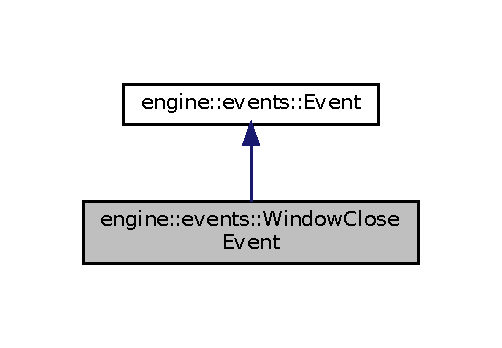
\includegraphics[width=227pt]{classengine_1_1events_1_1WindowCloseEvent__inherit__graph}
\end{center}
\end{figure}


Collaboration diagram for engine\+:\+:events\+:\+:Window\+Close\+Event\+:
\nopagebreak
\begin{figure}[H]
\begin{center}
\leavevmode
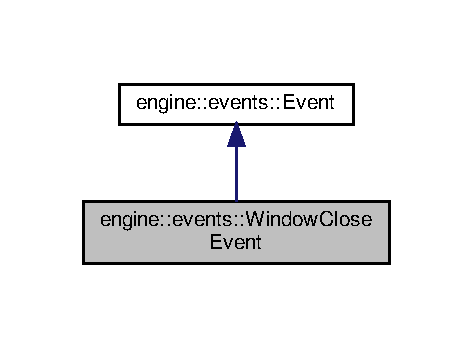
\includegraphics[width=227pt]{classengine_1_1events_1_1WindowCloseEvent__coll__graph}
\end{center}
\end{figure}
\subsection*{Additional Inherited Members}


The documentation for this class was generated from the following file\+:\begin{DoxyCompactItemize}
\item 
engine/src/core/events/Application\+Event.\+h\end{DoxyCompactItemize}

\hypertarget{structengine_1_1WindowProperties}{}\section{engine\+:\+:Window\+Properties Struct Reference}
\label{structengine_1_1WindowProperties}\index{engine\+::\+Window\+Properties@{engine\+::\+Window\+Properties}}


Generic \hyperlink{classengine_1_1Window}{Window} properties used to create platform specific windows.  




{\ttfamily \#include $<$Window.\+h$>$}

\subsection*{Public Member Functions}
\begin{DoxyCompactItemize}
\item 
\mbox{\Hypertarget{structengine_1_1WindowProperties_a8987e75ecc92e10f6764c0a677839b71}\label{structengine_1_1WindowProperties_a8987e75ecc92e10f6764c0a677839b71}} 
{\bfseries Window\+Properties} (const std\+::string \&title=\char`\"{}Game Engine\char`\"{}, unsigned int width=1280, unsigned int height=720)
\end{DoxyCompactItemize}
\subsection*{Public Attributes}
\begin{DoxyCompactItemize}
\item 
\mbox{\Hypertarget{structengine_1_1WindowProperties_a900cb8f590d355b520c7f8f4f75ecd99}\label{structengine_1_1WindowProperties_a900cb8f590d355b520c7f8f4f75ecd99}} 
std\+::string {\bfseries Title}
\item 
\mbox{\Hypertarget{structengine_1_1WindowProperties_a565d00a868bd2aae0abedb9e0f6faf9e}\label{structengine_1_1WindowProperties_a565d00a868bd2aae0abedb9e0f6faf9e}} 
unsigned int {\bfseries Width}
\item 
\mbox{\Hypertarget{structengine_1_1WindowProperties_aa88ea216a94e459a14c5e8549c9630ba}\label{structengine_1_1WindowProperties_aa88ea216a94e459a14c5e8549c9630ba}} 
unsigned int {\bfseries Height}
\end{DoxyCompactItemize}


\subsection{Detailed Description}
Generic \hyperlink{classengine_1_1Window}{Window} properties used to create platform specific windows. 

The documentation for this struct was generated from the following file\+:\begin{DoxyCompactItemize}
\item 
engine/src/core/\hyperlink{core_2Window_8h}{Window.\+h}\end{DoxyCompactItemize}

\hypertarget{classengine_1_1events_1_1WindowResizeEvent}{}\section{engine\+:\+:events\+:\+:Window\+Resize\+Event Class Reference}
\label{classengine_1_1events_1_1WindowResizeEvent}\index{engine\+::events\+::\+Window\+Resize\+Event@{engine\+::events\+::\+Window\+Resize\+Event}}


Generated whenever a window is resized.  




{\ttfamily \#include $<$Application\+Event.\+h$>$}



Inheritance diagram for engine\+:\+:events\+:\+:Window\+Resize\+Event\+:\nopagebreak
\begin{figure}[H]
\begin{center}
\leavevmode
\includegraphics[width=232pt]{classengine_1_1events_1_1WindowResizeEvent__inherit__graph}
\end{center}
\end{figure}


Collaboration diagram for engine\+:\+:events\+:\+:Window\+Resize\+Event\+:\nopagebreak
\begin{figure}[H]
\begin{center}
\leavevmode
\includegraphics[width=232pt]{classengine_1_1events_1_1WindowResizeEvent__coll__graph}
\end{center}
\end{figure}
\subsection*{Public Member Functions}
\begin{DoxyCompactItemize}
\item 
\mbox{\Hypertarget{classengine_1_1events_1_1WindowResizeEvent_ab3b3376d2bc9f18505798fc73ef35313}\label{classengine_1_1events_1_1WindowResizeEvent_ab3b3376d2bc9f18505798fc73ef35313}} 
{\bfseries Window\+Resize\+Event} (unsigned int width, unsigned int height)
\item 
unsigned int \hyperlink{classengine_1_1events_1_1WindowResizeEvent_a0858a751bbb0a18846c7377dbbe3d977}{Get\+Width} () const
\begin{DoxyCompactList}\small\item\em The new width that was registered with the event. \end{DoxyCompactList}\item 
\mbox{\Hypertarget{classengine_1_1events_1_1WindowResizeEvent_a1bde757195dac342cc7c1e1e8368a068}\label{classengine_1_1events_1_1WindowResizeEvent_a1bde757195dac342cc7c1e1e8368a068}} 
unsigned int {\bfseries Get\+Height} () const
\item 
\mbox{\Hypertarget{classengine_1_1events_1_1WindowResizeEvent_a7b51e15132e30f7e45cd045031a56afb}\label{classengine_1_1events_1_1WindowResizeEvent_a7b51e15132e30f7e45cd045031a56afb}} 
std\+::string {\bfseries To\+String} () const override
\end{DoxyCompactItemize}
\subsection*{Additional Inherited Members}


\subsection{Detailed Description}
Generated whenever a window is resized. 

Platform independent. 

\subsection{Member Function Documentation}
\mbox{\Hypertarget{classengine_1_1events_1_1WindowResizeEvent_a0858a751bbb0a18846c7377dbbe3d977}\label{classengine_1_1events_1_1WindowResizeEvent_a0858a751bbb0a18846c7377dbbe3d977}} 
\index{engine\+::events\+::\+Window\+Resize\+Event@{engine\+::events\+::\+Window\+Resize\+Event}!Get\+Width@{Get\+Width}}
\index{Get\+Width@{Get\+Width}!engine\+::events\+::\+Window\+Resize\+Event@{engine\+::events\+::\+Window\+Resize\+Event}}
\subsubsection{\texorpdfstring{Get\+Width()}{GetWidth()}}
{\footnotesize\ttfamily engine\+::events\+::\+Window\+Resize\+Event\+::\+Get\+Width (\begin{DoxyParamCaption}{ }\end{DoxyParamCaption}) const\hspace{0.3cm}{\ttfamily [inline]}}



The new width that was registered with the event. 

The new height that was registered with the event. 

The documentation for this class was generated from the following file\+:\begin{DoxyCompactItemize}
\item 
engine/src/core/events/\hyperlink{ApplicationEvent_8h}{Application\+Event.\+h}\end{DoxyCompactItemize}

%--- End generated contents ---

% Index
\backmatter
\newpage
\phantomsection
\clearemptydoublepage
\addcontentsline{toc}{chapter}{Index}
\printindex

\end{document}
